\newpage
\chapter{The Large Hadron Collider and the ATLAS detector}
\label{LHC&ATLAS}

The physics described in this thesis exclusively uses data collected by the ATLAS (A Toroidal LHC Apparatus) detector from high-energy proton-proton collisions, accelerated and been collided by the Large Hadron Collider (LHC). In terms of achievable centre-of-mass energy, LHC is currently the most powerful particle accelerator. The structure, parameters, and principles of LHC and ATLAS, besides the complex sub-detecting system, is introduced in this chapter.

\section{The Large Hadron Collider}
\label{chap2:LHC}
LHC is a circular collider of hadrons with a circumference of 27 kilometres. This machine is installed in a tunnel located underground between 50 m and 175 m depth, and was built between 1984 and 1989 for the LEP $e^+e^-$ machine. In 2001, LEP was dismounted to give way to the LHC. It was designed to accelerate and collide proton beams into a centre-of-mass energy up to 14 TeV. It also accelerates and collides heavy ions, in particular lead nuclei (Pb), at 2.3 TeV per nucleon. Inside this circular accelerator, a set of protons (or ions) so-called bunch racing clockwise at near the speed of light (99.9999991\%) collides to another bunch speeding anticlockwise. The energy involved in the collisions is so high that in a sub-microscopic region at the heart of the collisions, it briefly generates conditions similar to those that occurred shortly after the birth of the universe. \\ 
Within the tunnel are two adjacent parallel beam pipes and surrounded by superconductive magnets. In total, 1232 dipole magnets bend the beams into their circular orbit and 392 quadrupole magnets corresponding to the function of beams focusing. The strength of the focusing magnets is required to be high to squeeze the transverse beam sizes and, thus, increase the probability of collisions. The adopted design at the LHC is approximately 80\% of the arcs is filled with dipole magnets. Dipoles are also equipped with sextupoles, octupoles and decapoles, functions of which is to correct non-linear dynamics of the beams.  Keeping 7 TeV proton energy beam on the designed orbit implies the use of magnetic bending fields of 8.4 T. Generation of such field required using superconducting magnets at the limit of the existing technologies. Approximately 96 tonnes of liquid helium is needed to maintain the superconductivity of the magnets at an operational temperature of 1.9 K (-271.3 C), making the LHC the largest cryogenic facility in the world.  A detailed description of the LHC and the CERN accelerator complex is given in Ref. \cite{LHCTDR}.

\subsection{Acceleration chain}
\label{chap2:LHC:chain}
A succession of small to large accelerators is used to accelerate the protons extracted from hydrogen gas to the energy needed for injection into the LHC. Figure \ref{fig:chap2:LHC:chain} displays the CERN accelerator complex including all pre-acceleration steps before the LHC. 
\begin{figure}[htbp]
    \centering
    \includegraphics[width=\textwidth]{Ch2/Img/LHC_chain.jpeg}
    \caption{Overview of the CERN accelerator complex, including the LHC and its pre-accelerators \cite{LHC_chain}. The four main LHC experiments are depicted, too.}
    \label{fig:chap2:LHC:chain}
\end{figure}
\\
The process of acceleration starts from the linear accelerator Linac 2, which accelerates protons up to 50 MeV. The beam is then injected into the Booster. The Booster accelerates the beam to 1.4 GeV and feeds the Proton Synchrotron (PS), where protons are further accelerated to 25 GeV. The next chain is the Super Proton Synchrotron (SPS), which is 6.9 km long. Here protons reach the energy of 450 GeV before they are transferred to two beam-pipes of the LHC main ring. It takes several minutes to fill the LHC ring and about 15 minutes to accelerate beams to their maximum energy of 6.5 TeV using eight radio frequency (RF) cavities at $f_{RF} = 400$ MHz. Each time a beam passes the electric field in the RF cavity, some energy from the radio waves is transferred to the particles, nudging them forwards. The beams are injected in bunches spaced by 25 ns. Each bunch contains approximately $10^{11}$ protons. Each beam contains 2808 bunches. \\
Particles created in LHC collisions are distributed over the full solid angle around the Interaction Point (IP), in four IP points is installed four detectors to record those particles and identified them as ATLAS, CMS, ALICE and LHCb. LHCb was built to study flavour physics looking at the properties of $b$-hadrons, and the ALICE detector is specialized for measurements on heavy-ion collisions. CMS and ATLAS are general-purpose detectors. They allow making precision measurements of SM processes, including the properties of the Higgs boson, and to search for BSM physics. Section \ref{chap2:ATLAS} is dedicated to ATLAS detector.

\subsection{Luminosity}
\label{chap2:LHC:Lumi}
The number of produced events is proportional to the integrated luminosity $\mathcal{L}_{int}$ multiplied by the total cross-section: 
\begin{equation}
N_{events} = \int\mathcal{L} dt \times \sigma_{process}.
\end{equation}
The instantaneous luminosity $\mathcal{L}$ is the quality factor for colliders, measuring the intensity of the beam, and is defined as:
\begin{equation}
\mathcal{L} = \frac{N_b^2n_bf_r\gamma_r}{4\pi\epsilon_n\beta^*}F,
\end{equation}
where for the design luminosity (nominal parameters for the LHC are given in parentheses):
\begin{itemize}
	\item $N_b$ is the number of particle per bunch ($\sim10^{11}$).
	\item $n_b$ is the number of bunch per beam (2808).
	\item $f_r$ is the revolution frequency (11245 Hz).
	\item $\gamma_r$ is the relativistic $\gamma$ factor ($\sim 7000$).
	\item $\epsilon_n$ is the normalized traverse beam emittance which characterizes its spread in coordinate and momentum phase space (3.75 $\mu$m).
	\item $\beta^*$ is the beta function at the collision point determined by the magnet configuration (for ATLAS 0.55 m).
	\item $F$ is the geometric luminosity reduction factor due to the crossing angle at the interaction point.
\end{itemize}
For optimizing the analysis procedure, ATLAS has defined a basic time unit called Luminosity Block (LB) where the luminosity is assumed to be stable. The typical LB duration is one to two minutes. Data are analysed under the assumption that each LB contains data taken under uniform conditions (data quality). To define a data sample for physics, quality criteria are applied to select LBs where the conditions are acceptable. The average luminosity in the LB is multiplied by the LB duration to provide the integrated luminosity delivered in the given LB. \\
The design luminosity of LHC is $10^{34} \ cm^{-2}s^{-1}$. The integrated good quality data of Run-1 is approximately 25 \ifb as shown in Figure \ref{fig:chap2:LHC:Lumi:Run1}, which Higgs self-coupling measurement does not benefit from it because of the low $\sigma_{pp\rightarrow HH}$. During the first long shutdown (LS1), the LHC beam energy is increased from 3.5 TeV to 6.5 TeV which increases the luminosity. 
\begin{figure}[htbp]
    \centering
    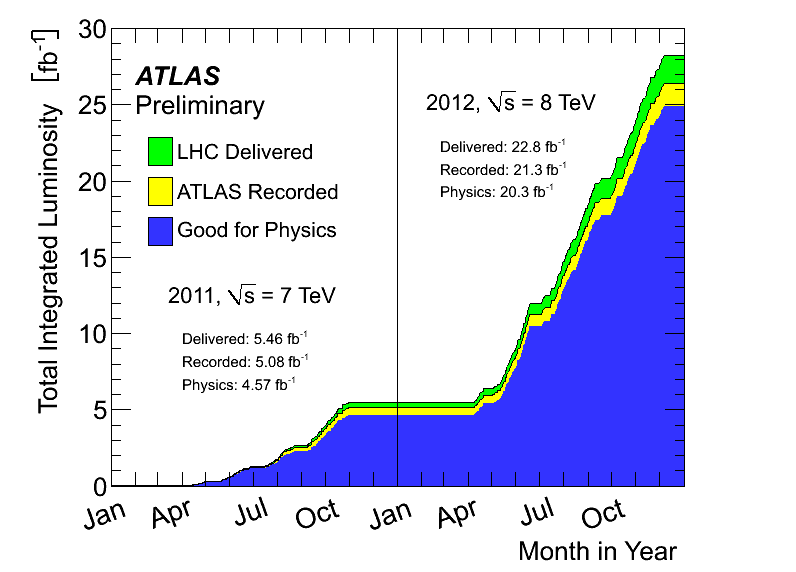
\includegraphics[width=0.5\textwidth]{Ch2/Img/LumiRun1.png}
    \caption{Cumulative luminosity versus time delivered to (green), recorded by ATLAS (yellow), and certified to be good quality data (blue) during stable beams and for pp collisions at 7 and 8 TeV centre-of-mass energy in 2011 and 2012 (Run-1).}
    \label{fig:chap2:LHC:Lumi:Run1}
\end{figure}
Figure \ref{fig:chap2:LHC:Lumi} shows the delivered and recorded luminosity during the Run-2 data taking \cite{Lumi2018}. The integrated luminosity of Run-2 corresponding to good data period is $\mathcal{L}_{int} = 139 $ \ifb. The analysis described in this thesis is performed with Run-2 data.\\
\begin{figure}[htbp]
    \centering
    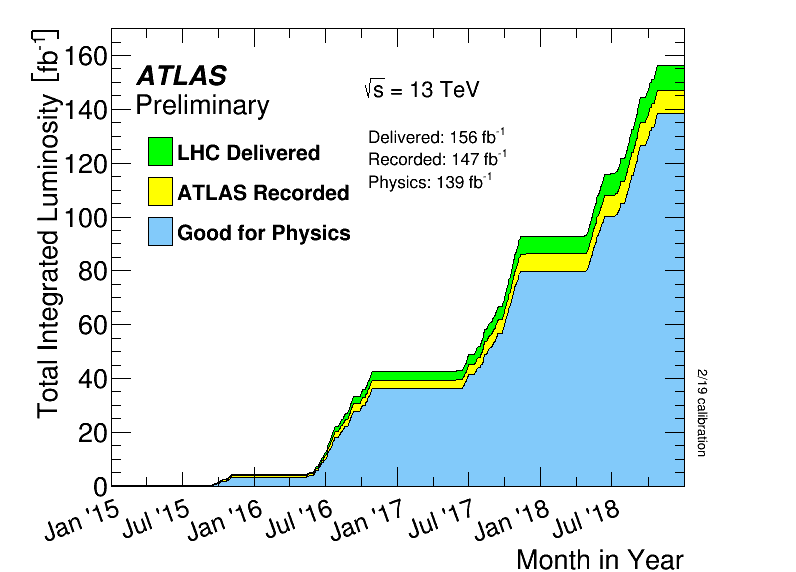
\includegraphics[width=0.6\textwidth]{Ch2/Img/Lumi.png}
    \caption{Luminosity delivered by the LHC during the Run-2 data taking. ATLAS recorded this data with an efficiency above 90\%.}
    \label{fig:chap2:LHC:Lumi}
\end{figure}
\\
Knowing the cross-section of the \HHyybb production, one can evaluate the number of events available for the analysis as $N_{HH\rightarrow\gamma\gamma\bar{b}b} = \mathcal{L}_{int}\cdot\sigma_{pp\rightarrow HH}\cdot Br(HH\rightarrow\gamma\gamma\bar{b}b)$ that leads to about 12 events.

\subsection{Pile-up events}
\label{chap2:LHC:PU}
Because of the very high proton density at the collision points, more than one proton interact when two LHC bunches cross each other at the centre of the experiment. This is commonly referred to as "pile-up". On top of the usual \textit{in-time} pile-up, defined as the collision events occurring during the same bunch-crossing as the event of interest, one also has to consider \textit{out-of-time} pile-up, coming from remnants of information found in some of the detector subsystems that end up being attributed to the wrong bunch-crossing, and therefore to the wrong event typically from previous collisions. Figure \ref{fig:chap2:LHC:PU} shows the average number of simultaneous interactions per bunch crossing for Run-2. \\
\begin{figure}[htbp]
    \centering
    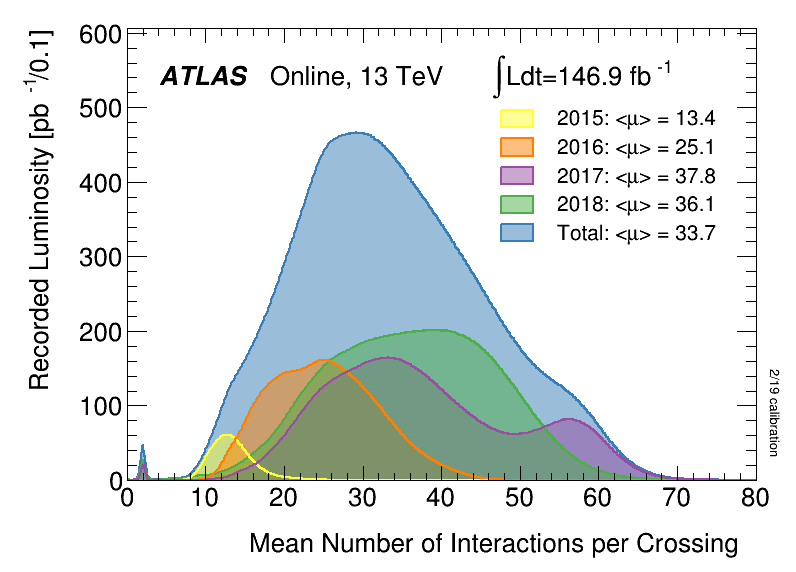
\includegraphics[width=0.6\textwidth]{Ch2/Img/PU.png}
    \caption{Recorded integrated luminosity as function of the mean number of interaction per bunch crossing in pp collisions recorded by the ATLAS detector during Run-2 \cite{Lumi2018}.}
    \label{fig:chap2:LHC:PU}
\end{figure}

\section{ATLAS : A Toroidal LHC ApparatuS detector}
\label{chap2:ATLAS}
The ATLAS detector is one of the four experiments placed on the crossing points of the LHC beams. It is currently the largest experiment of particle physics with a length of 46 m along the beam pipe and a transverse diameter of 25 m. Its weight is more than 7000 tons \cite{ATLAS_Exp}. It is a superposition of four sub-detectors, each optimized for the identification and the measurement of a specific category of particles: Inner Tracker, Electromagnetic Calorimeter (ECAL), Hadronic Calorimeter (HCAL) and Muons Spectrometer. It is composed of a central component called Barrel and two End-Cap to cover the $4\pi$ solid angle. Its geometry is optimized to detect particles produced orthogonally to the beam pipe and allow for forwarding detection to estimate the energy of invisible particles. The detector has been operating since 2008, taking alignment data with cosmic rays before the LHC launches, and its data is exploited by a collaboration of about 3000 scientific authors from 181 institutions in 38 countries. An overview sketch of the ATLAS detector is shown in Figure \ref{fig:chap2:ATLAS:Img}.
\begin{figure}[htbp]
    \centering
    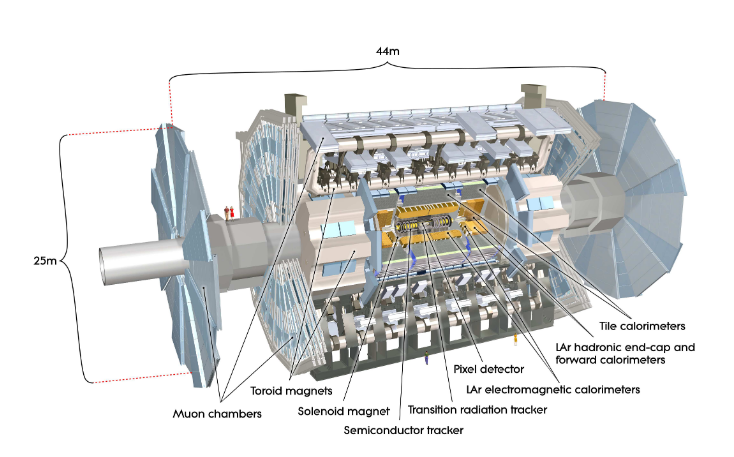
\includegraphics[width=0.8\textwidth]{Ch2/Img/ATLAS_sketch.png}
    \caption{Sketch of the ATLAS detector with its different sub-detectors.}
    \label{fig:chap2:ATLAS:Img}
\end{figure}

\subsection{System of coordinates}
\label{chap2:ATLAS:CS}
The coordinate system used in the ATLAS experiment is the cylindrical one where the z-axis is along the LHC beam pipe, the x-axis pointing toward the centre of the LHC ring and the y-axis pointing upward. A physic object (particle) is identified by its transverse component of the three-momentum $p_T = \sqrt{p_X^2 + p_Y^2}$, its azimuthal angle $\phi \in [-\pi,\pi] $ formed by the three-momentum and the x-axis and its polar angle $\theta \in [0,\pi]$, i.e., the angle between the three-momentum and the z-axis. \\
The polar angle is expressed in terms of the pseudo-rapidity $\eta$, defined as:
\begin{equation}
\eta = -\log[\tan(\theta/2)].
\end{equation}
In collisions involving protons, the adoption of $\eta$ instead of $\theta$ ensure the detector balance over particles and particles distribution recorded is approximately flat in $\eta$:
\begin{equation}
\frac{\partial\sigma_{QCD}}{\partial\eta} = cte.
\end{equation}
The pseudo-rapidity $\eta$ coincides for relativistic particles to the rapidity $y$, defined as:
\begin{equation}
y = \frac{1}{2}(\frac{E+p_Z}{E-p_Z}),
\end{equation}
where E is the particle energy.
Figure \ref{fig:chap2:ATLAS:SYS} shows the coordinate system common to ATLAS and CMS experiments.
\begin{figure}[htbp]
    \centering
    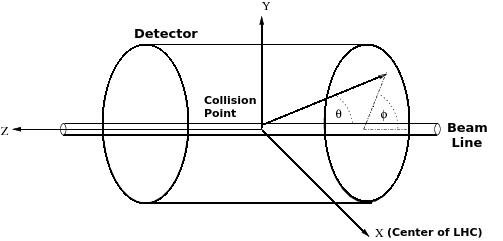
\includegraphics[width=0.6\textwidth]{Ch2/Img/ATLAS_Sys.jpeg}
    \caption{Coordinate system used by the ATLAS and CMS experiments at the LHC.}
    \label{fig:chap2:ATLAS:SYS}
\end{figure}

\subsection{Inner Tracker}
\label{chap2:ATLAS:ITk}
The Inner Detector (ID) has been designed to detect and reconstruct the path of the electrically charged particle bent by a 2 T solenoid magnetic field. It also provides a good momentum resolution by reconstructing the curvature and the direction, and both primary and secondary vertex measurements for tracks above approximately 0.5 GeV \cite{ID_TRD, TrkVertexing}. In terms of acceptance, the ID covers the region of $|\eta|\leqslant2.5$. To achieve the momentum and vertex resolution requirements imposed by the physics goals at the LHC and the very large track density environment, the ID high-precision measurements must be made with fine detector granularity. The ID is composed of four complementary sub-detectors: IBL, the Pixel Detector, the Semi-Conductor Tracker (SCT) and the Transition Radiation (TRT). A magnetic field of 2 T is provided by a solenoid inserted between the ID and the EM calorimeter. The layout of the Inner Detector (ID) is illustrated in Figure \ref{fig:chap2:ATLAS:ITK:ID}.
\begin{figure}[htbp]
    \centering
    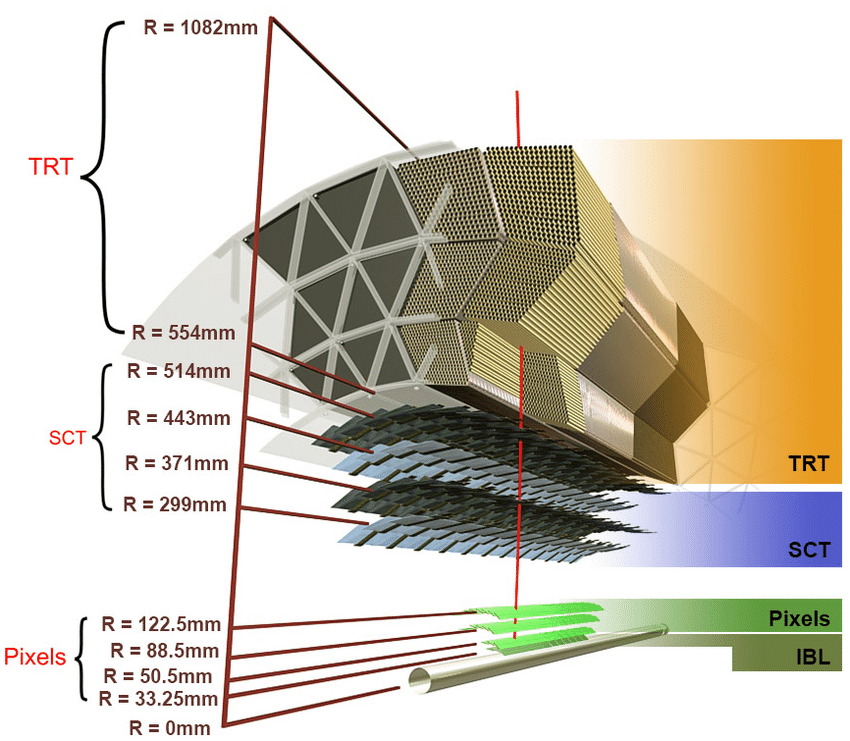
\includegraphics[width=0.5\textwidth]{Ch2/Img/ID_withIBL.png}
    \caption{Layout of the Inner Detector (ID) \cite{ID_withIBL}.}
    \label{fig:chap2:ATLAS:ITK:ID}
\end{figure}

\subsubsection{IBL}
\label{chap2:ATLAS:ITK:IBL}
In 2014, during the first LHC long shutdown (LS1), the ATLAS pixel detector was upgraded with a pixel layer installed close to the beam pipe called Insertable B-Layer (IBL) \cite{IBL_TDR}. Its motivations are:
\begin{itemize}
    \item Increase the number of measurement point of tracks to improve their reconstruction efficiency.
	\item Improve the identification of the primary vertex which plays an important role in $b$-jet identification ($b$-tagging), which in turn significantly improves the sensitivity of many analyses. Inefficiencies in the other layers can be partially compensated during the reconstruction at the cost of an increased fake rate, the IBL restore the full $b$-tagging efficiency even in case of a complete B-layer failure.
	\item Luminosity effects: The pre-Run-2 pixel detector was designed for a peak luminosity of $10^{34} \ cm^{-2}s^{-1}$. With high luminosity the number of tracks from pile-up is increased, leading to high occupancy that can induce readout inefficiencies, would thereby limit the $b$-tagging efficiency. The addition of the IBL layer helps to preserve tracking performance in face of luminosity increase.
\end{itemize}
Strong constraints and project specifications have a substantial impact on the technologies required for the IBL. IBL covers the region of $|\eta| < 2.58$ and located at a mean radius of 33.2 mm around the beam pipe. The typical size of IBL pixels is 50$\times$250 $\mu$m. The IBL consists of 14 staves with every 20 modules made using planar sensors. The temperature of the IBL is controlled using a bi-phase $CO_2$ cooling system. Figure \ref{fig:chap2:ATLAS:ITK:IBL} shows the IBL within the Pixel Detector volume and around the beam pipe.
\begin{figure}[htbp]
    \centering
    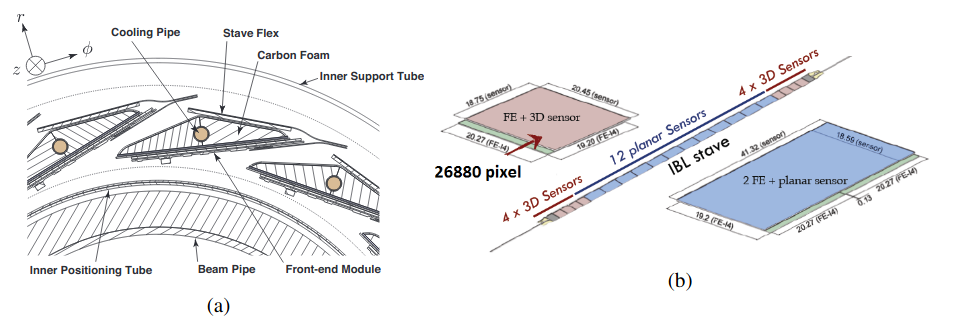
\includegraphics[width=0.8\textwidth]{Ch2/Img/IBL.png}
    \caption{(a) Transverse view of 3 of the Insertable-B-Layer (IBL) staves, located directly on the beam pipe. (b) The layout of one of the 14 IBL staves \cite{ID_withIBL}.}
    \label{fig:chap2:ATLAS:ITK:IBL}
\end{figure}
\\
The additional measurement point provided by IBL improves significantly the reconstructed parameters by the tracker. Figure \ref{fig:chap2:ATLAS:ITK:IBL:Imp} shows the improvement in impact parameter resolution due to the IBL as measured from early Run-2 data with respect to Run-1. 
\begin{figure}[htbp]
    \centering
    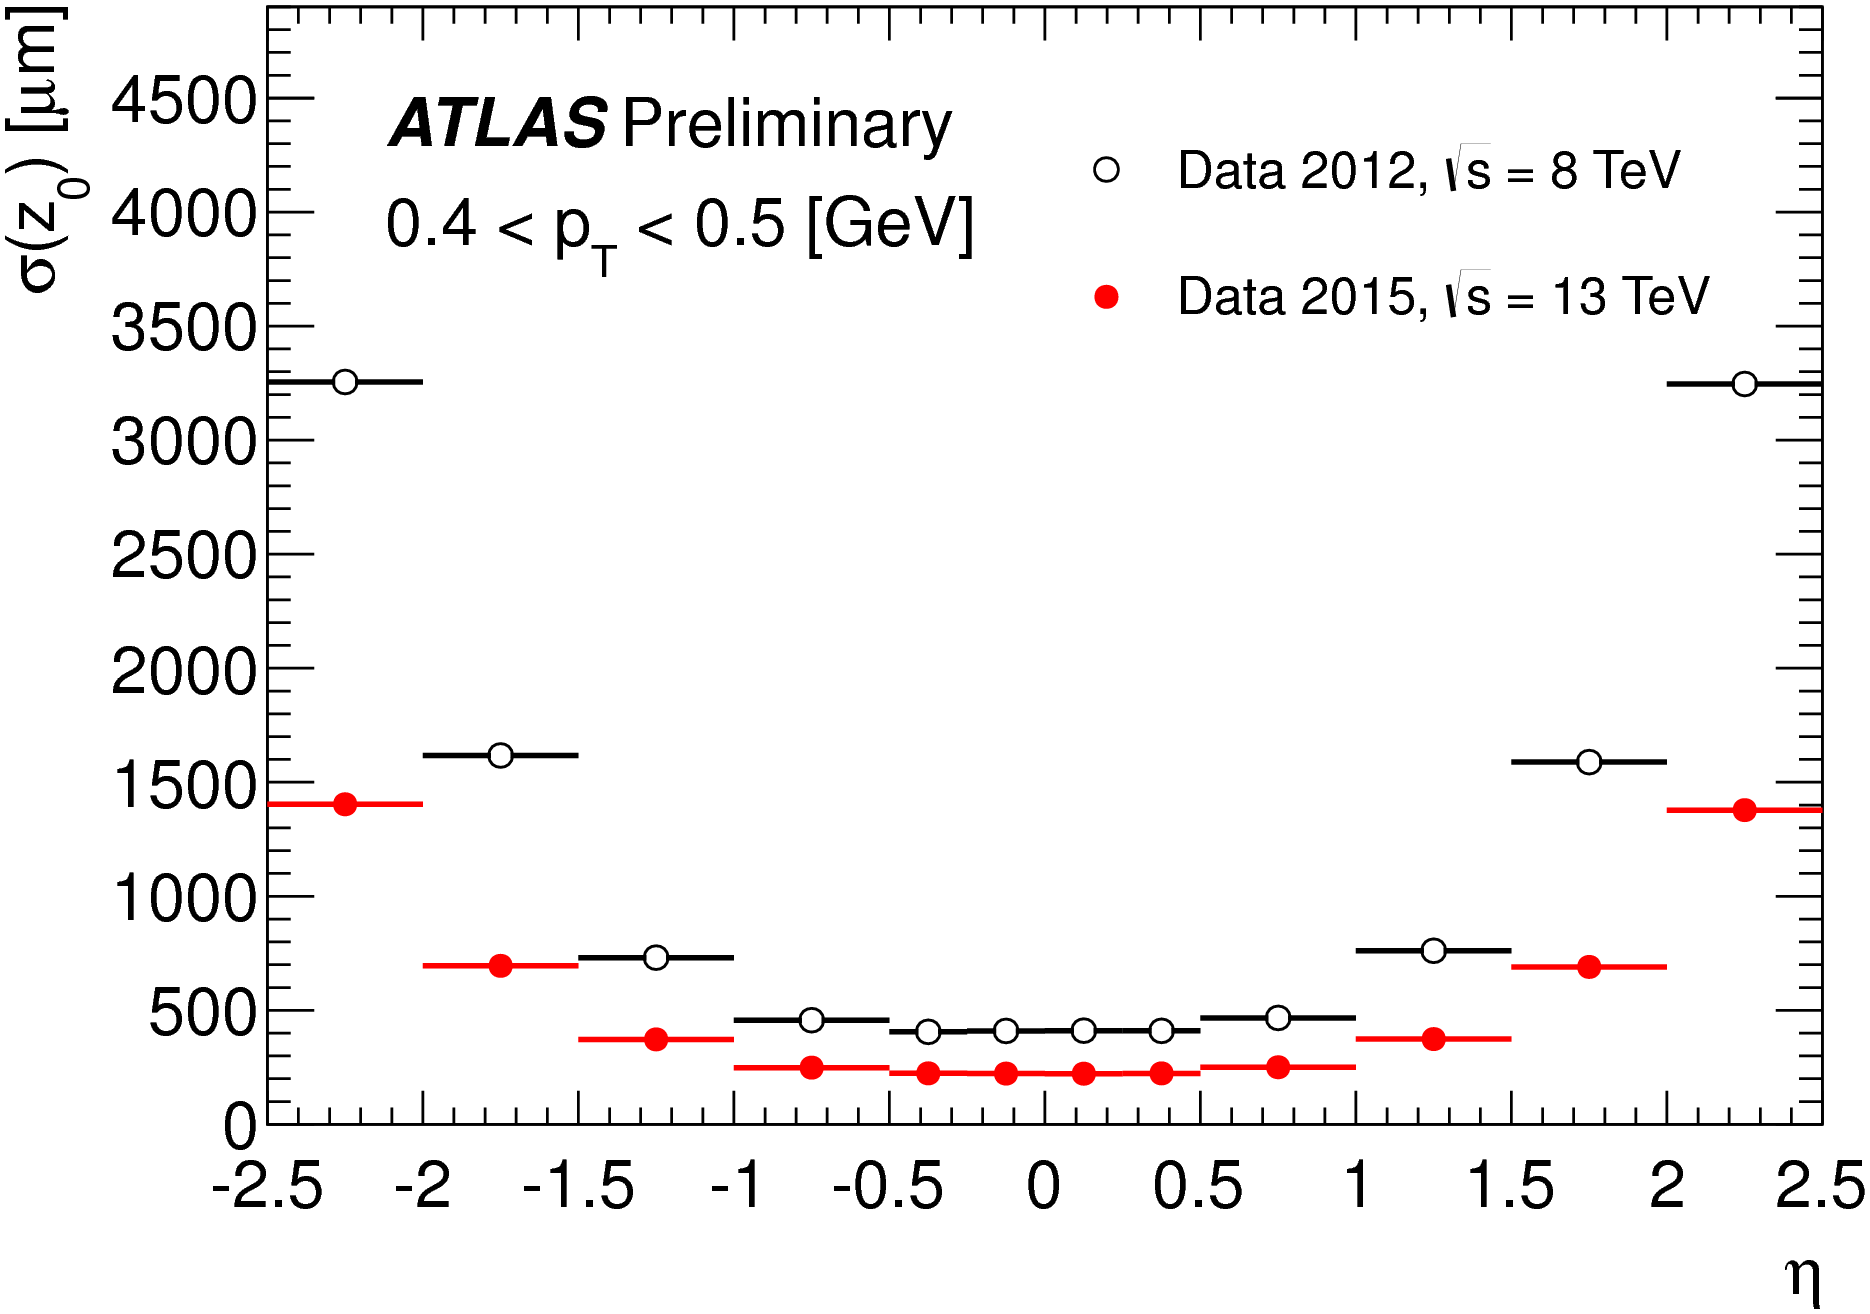
\includegraphics[width=0.6\textwidth]{Ch2/Img/IBL_impact.png}
    \caption{Unfolded longitudinal impact parameter resolution measured from data in 2015, $\sqrt{s}= 13$ TeV, with the Inner Detector including the IBL, as a function of $\eta$  for values of $0.4 < p_{T} < 0.5$ GeV compared to that measured from data in 2012 \cite{IBL_IP}.}
    \label{fig:chap2:ATLAS:ITK:IBL:Imp}
\end{figure}
In addition to a factor of 4 reduction in reconstruction speed \cite{IBL_Time}, Figure \ref{fig:chap2:ATLAS:ITK:IBL:Trk} shows the improvement achieved with IBL for the performance of tracking in dense environments (TIDE). Improvements in tracking have a direct impact on vertex identification and $b$-tagging. 
\begin{figure}[htbp]
    \centering
    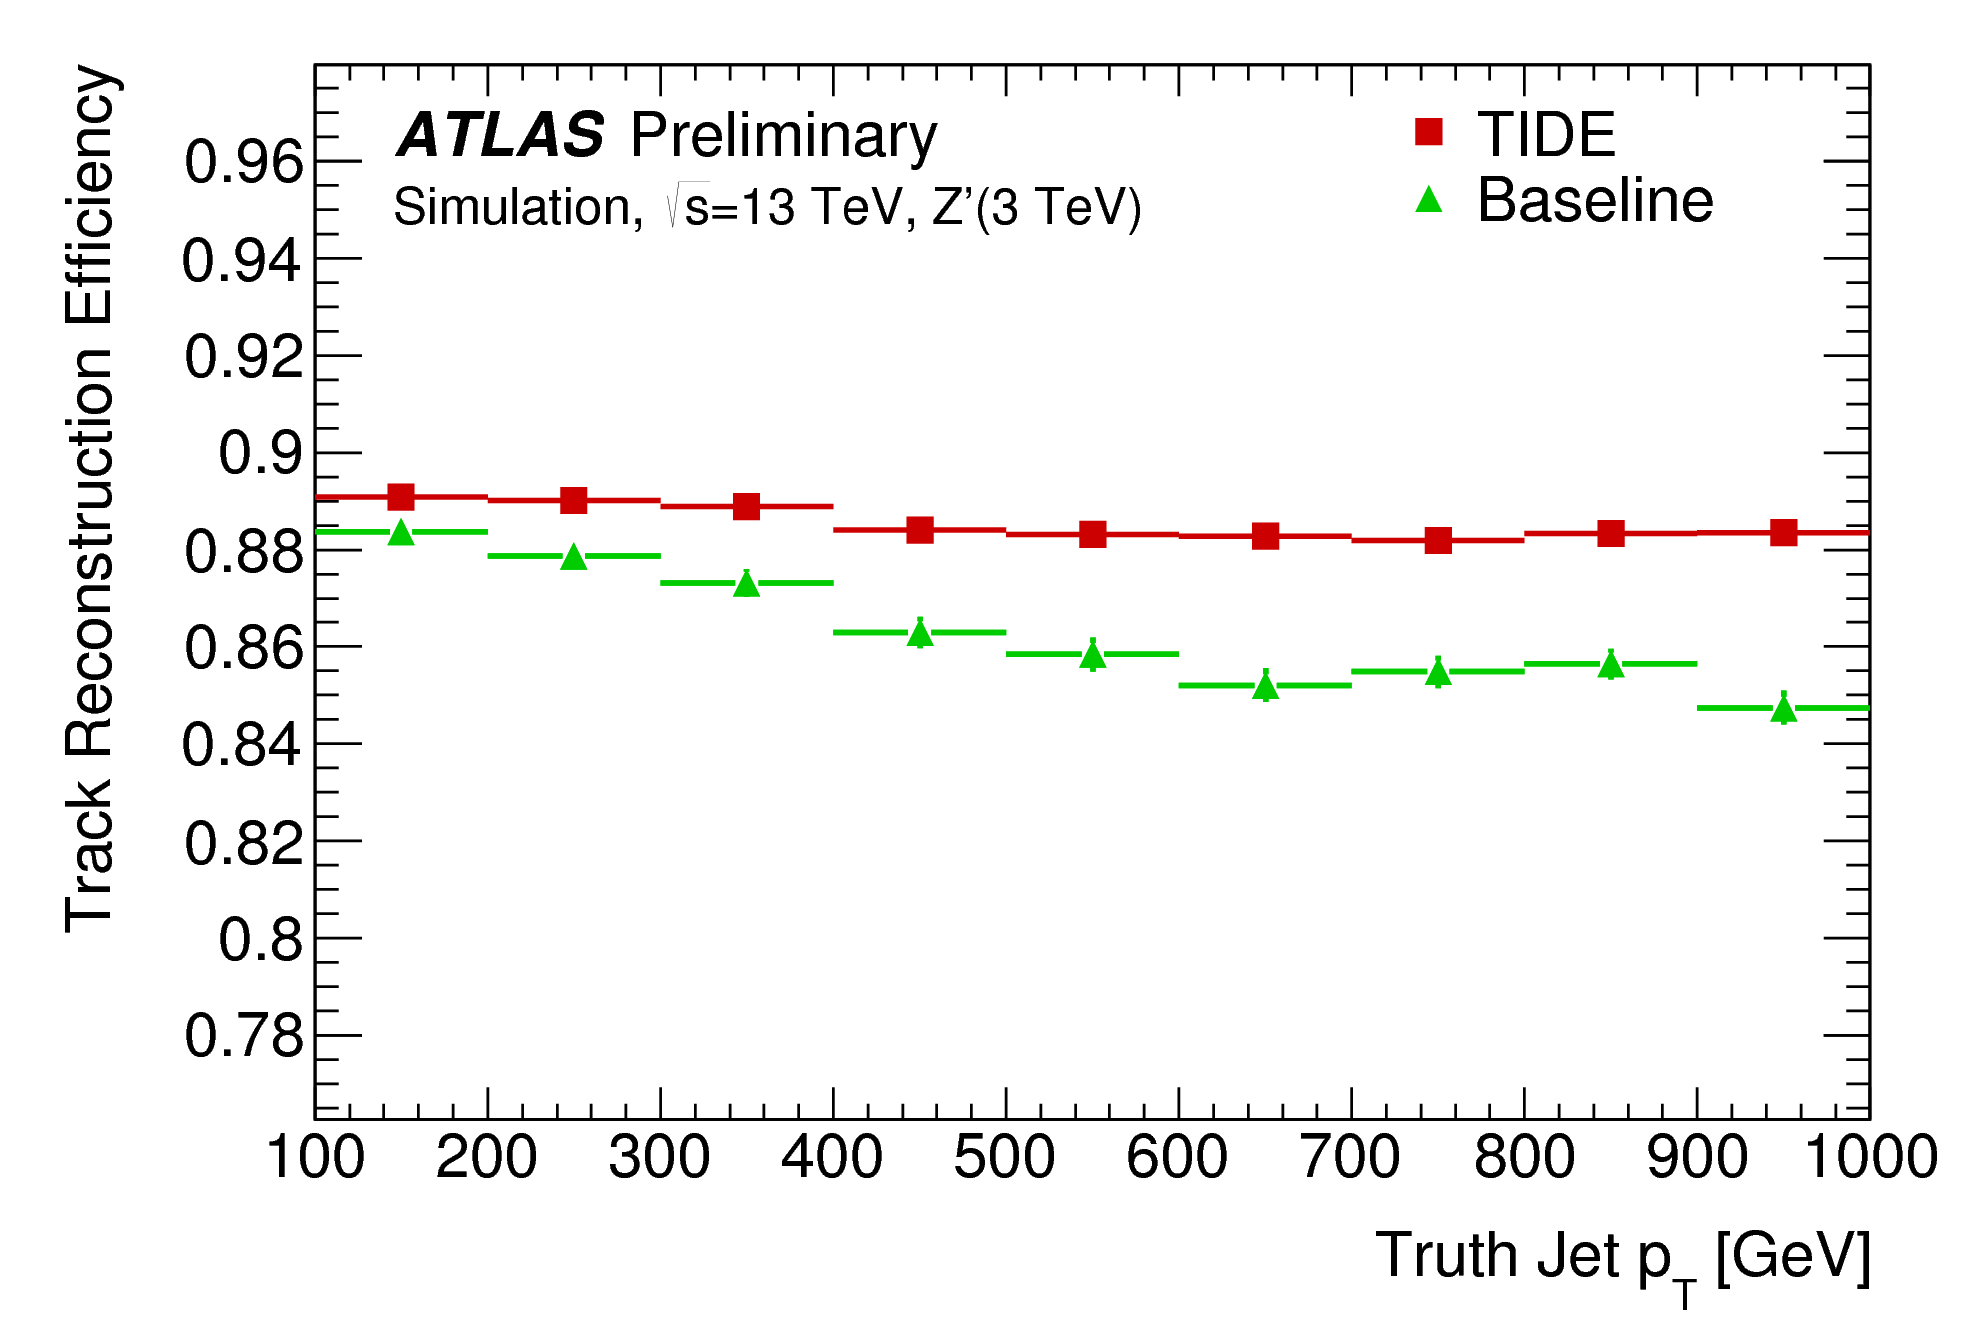
\includegraphics[width=0.6\textwidth]{Ch2/Img/IBL_track.png}
    \caption{The average efficiency to reconstruct primary tracks with a production vertex before the first layer in jets as a function of jet \pT. The same sample generation, with limited statistics, is used for both reconstruction algorithms, resulting in correlated features \cite{IBL_Trk}.}
    \label{fig:chap2:ATLAS:ITK:IBL:Trk}
\end{figure}
Figure \ref{fig:chap2:ATLAS:ITK:IBL:Btag} shows the improvement in the $b$-tagging efficiency with IP3D+SV1 $b$-tagging algorithms in respect to Run-1 algorithm due to the IBL and new algorithm \cite{IBL_Btag, IBL_Btag2}. The IP3D and SV1 algorithms will be explained later in the thesis.
\begin{figure}[htbp]
    \centering
    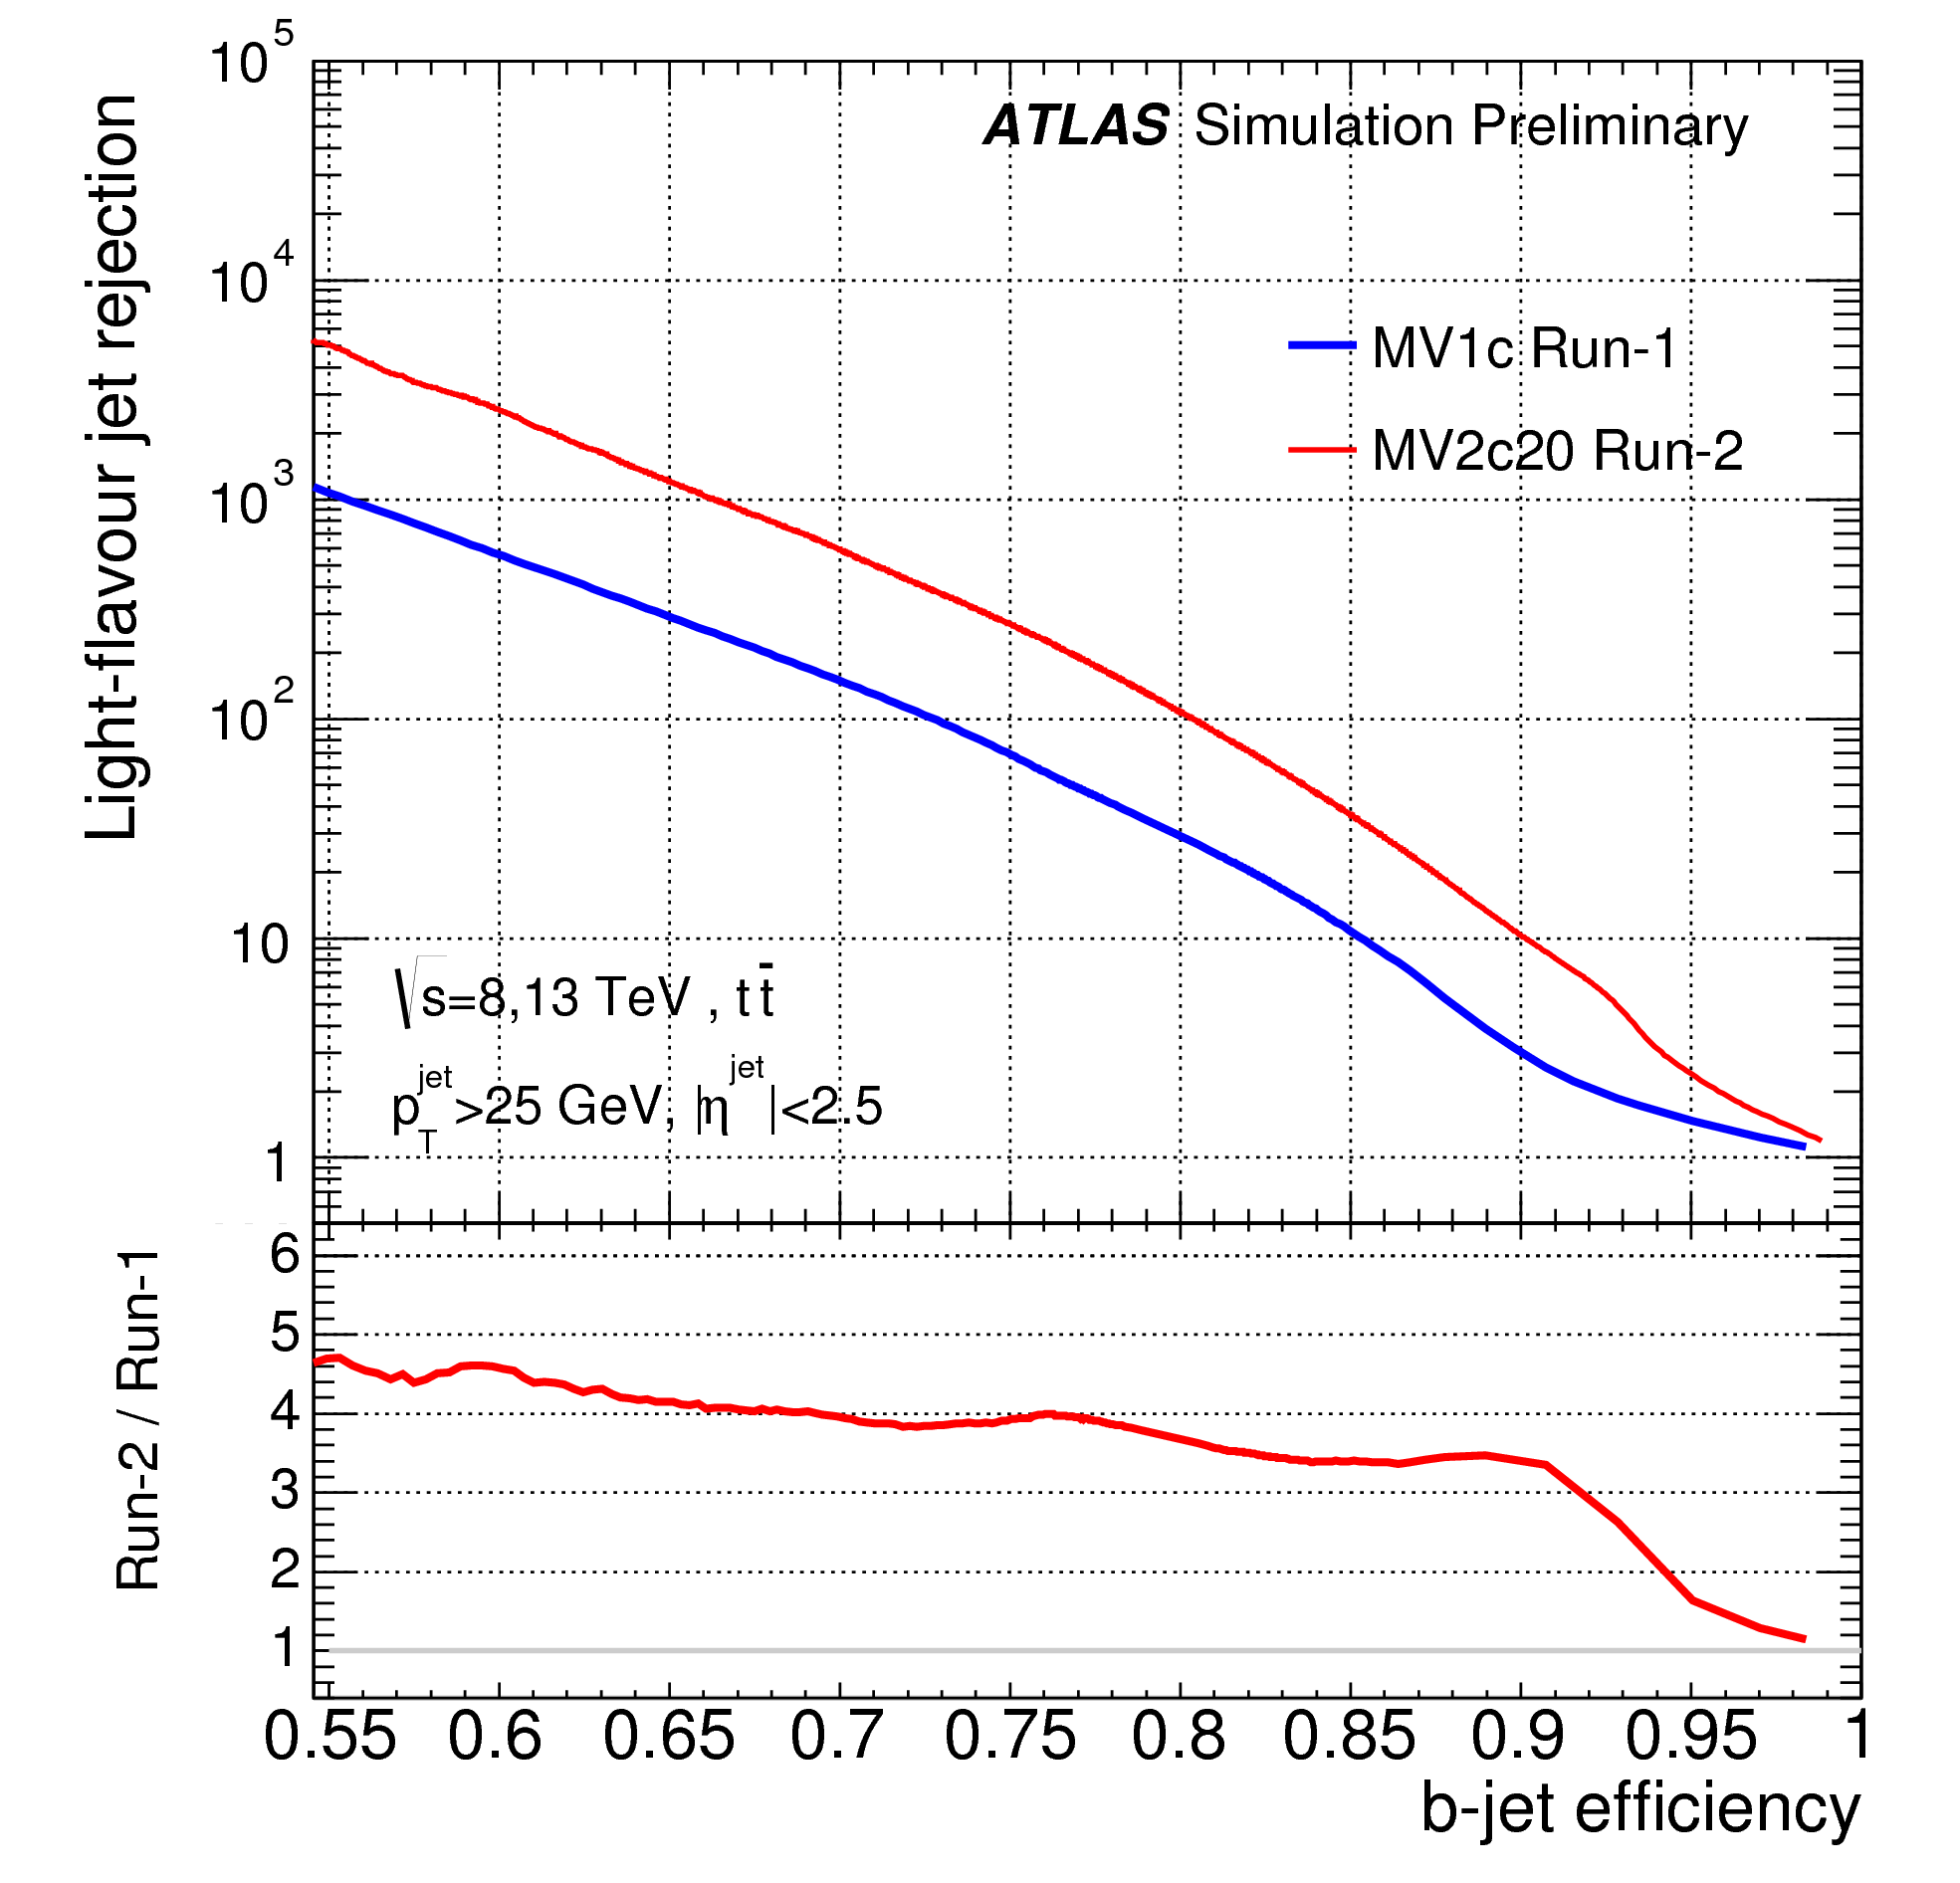
\includegraphics[width=0.6\textwidth]{Ch2/Img/IBL_btag2.png}
    \caption{Rejection factor against light jets as a function of $b$-jet efficiency for t the combined IP3D+SV1 tagger. Compared are the results with and without IBL.}
    \label{fig:chap2:ATLAS:ITK:IBL:Btag}
\end{figure}

\subsubsection{Pixel Detector}
\label{chap2:ATLAS:ITK:PD}
With the existing technology at that time (2000s), the Pixel Detector (PD) installed before Run-1 was designed to provide high-granularity, high-precision measurements as close as possible to the interaction point. It consists of three barrel layers placed at the radius of 50.5 mm, 88.5 mm and 122.5 mm centred around the beam axis and two end-cap with three disc layers each positioned at $|z|=$ 495.580 and 650 mm. It provides three measurement points per track. The system is designed to be highly modular, containing approximately 1500 identical barrel modules and 1000 identical disk modules, each module is composed of 61440 pixel elements of silicon semi-conductor. In total there are about 80 million readout channels in the whole PD. The spatial resolution for the barrel modules is 10 $\mu$m in r-$\phi$ and 66 $\mu$m in z, for the end-caps the spatial resolution in r-$\phi$ is the same as the barrel and 115 $\mu$m in z. The main limitation of the pixel detector is the radiation hardness, as the expected flounce is at the tolerable limit. 

\subsubsection{Semi-Conductor Tracker}
\label{chap2:ATLAS:ITK:SCT}
The SCT system is designed to provide four precision points per track in the intermediate radial range, contributing to the measurement of momentum, impact parameter and vertex position. The barrel and end-caps SCT are four layers of silicon microstrip for barrel and nine disks for end-caps. The spatial resolution is 16 $\mu$m in r-$\phi$ for both the barrel and the end-caps. The four complete barrels are positioned in a radius of 300, 373, 447 and 520 mm. Tracks can be distinguished if separated by more than $\sim$ 200 $\mu$m. There are 6.3 millions readout channels for the SCT.

\subsubsection{Transition Radiation Tracker}
The TRT is positioned at the outer part of the ID. It consists of 370000 drift tubes called straws. Each straw has a diameter of 4 mm and 1.44 m in long. The straws are filled with a gas mixture of 70\% $Xe$, 27\% $CO_2$ and 3\% $O_2$. Its wall acts as a cathode and kept at high voltage. The anode is a 30 $\mu$m diameter plated tungsten wire placed in the centre of the straw. When a charged particle traverses a straw, it ionizes the gas and the produced electrons travel through the anode generating an electric signal. To keep the TRT performance constant, the close-loop gas system is used, maintaining the correct gas fractions. The straws are arranged to be parallel to the beam-pipe in the barrel and perpendicular in the end-cap region. There are about 50k straws in the barrel and 320k straws in the end-cap providing high-precision measurement for each track. The radial resolution is about 130 $\mu$m. \\

In the Perigee representation, tracks are described using the parameters of a helical trajectory at the point of the closest approach to the z-axis: the transverse impact parameter $d_0$, the z coordinate $z_0$, the angles $\theta$ and $\phi$ and the inverse of the particle momentum multiplied by the charge q/p, as illustrated in Figure \ref{fig:chap2:ATLAS:ITK:Trk}.
\begin{figure}[htbp]
    \centering
    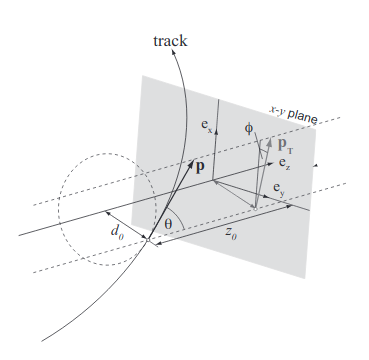
\includegraphics[width=0.5\textwidth]{Ch2/Img/Track.png}
    \caption{The Perigee representation of the track \cite{Track_schema}.}
    \label{fig:chap2:ATLAS:ITK:Trk}
\end{figure}
\\
The expected momentum resolution of the inner detector, without the IBL, is given by:
\begin{equation}
    \sigma(1/p_T)\cdot p_T = 0.036\%\cdot p_T [GeV] \oplus 1.3\%,
\end{equation}
$\oplus$ denote the quadrature addition.

\subsection{Calorimeter system}
\label{chap2:ATLAS:Calo}
Based on the calorimetry, the ATLAS calorimeter system is designed to provide a precise energy measurement and position reconstruction for electromagnetic (EM) particles (electrons, photons) and jets (hadrons). The good hermiticity of the calorimeter ($|\eta|$ up to 5) also allows to measure the missing transverse energy and provides the separation of electrons and photons from hadrons and jets. The calorimeter system is composed of two calorimeters: the electromagnetic calorimeter (ECal) and the hadronic calorimeter (HCal). Both are sampling calorimeters, with alternating layers of a heavy absorber material and an active material in which an ionization signal is produced. Figure \ref{fig:chap2:ATLAS:Calo} shows a three-dimensional view of the ATLAS calorimeter system.
\begin{figure}[htbp]
    \centering
    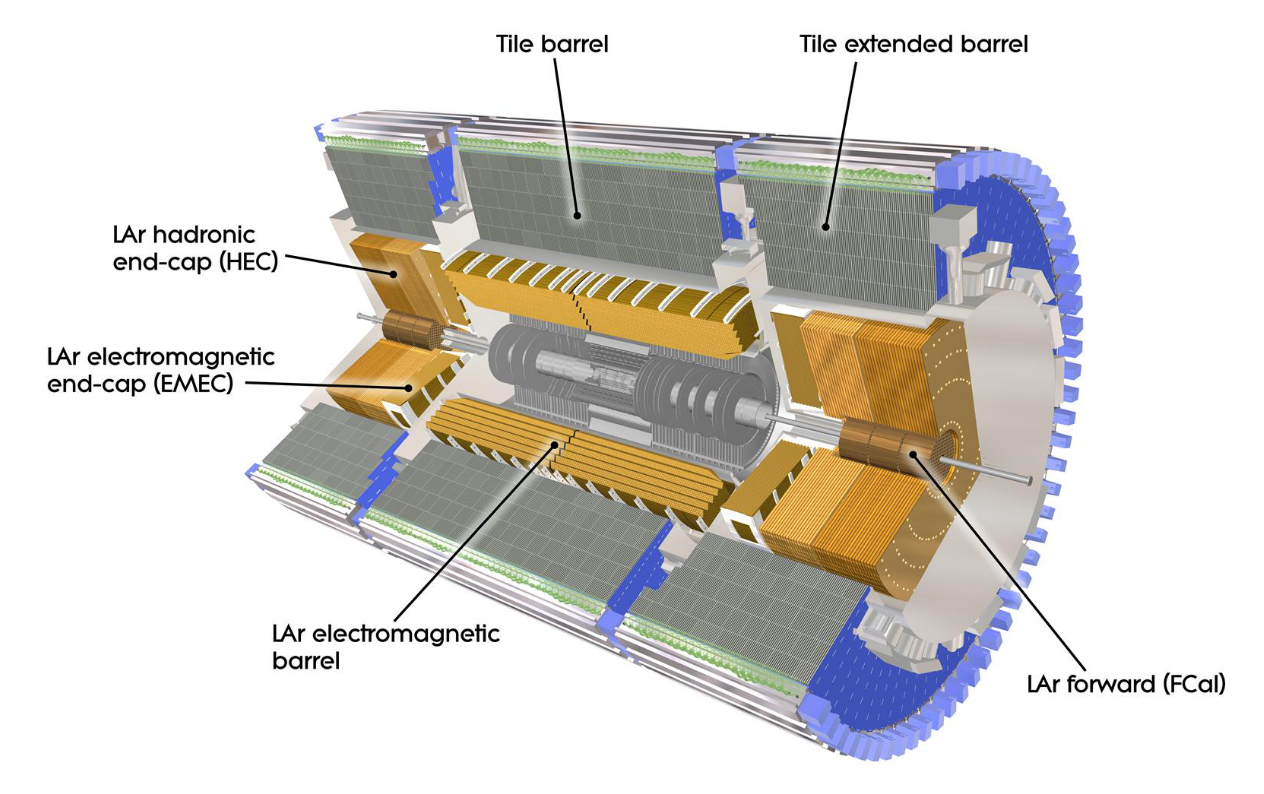
\includegraphics[width=0.6\textwidth]{Ch2/Img/Calo.png}
    \caption{ATLAS Calorimeter system.}
    \label{fig:chap2:ATLAS:Calo}
\end{figure}

\subsubsection{Electromagnetic calorimeter}
\label{chap2:ATLAS:Calo:ECAL}
The ECal is the first sub-detector after the ID. It is optimized for the energy reconstruction of electrons and photons by triggering EM shower and measure its properties \cite{LAr_TRD}. It covers the region of $|\eta| < $ 3.2 excluding the region 1.375 $ < |\eta| < $ 1.52 which corresponds to the transition region between the barrel and end-caps. The barrel part covers $|\eta| < $ 1.475, while the two end-caps cover 1.375$ < |\eta| < $ 3.2. The barrel and end-caps are composed of alternated layers of absorbing material lead (Z = 82) plates ($\sim$ 1 mm thick), to enforce the development of the full EM showers within EM longitudinal envelop and separated by active medium Liquid Argon (LAr) of 2 mm thick. The advantages of LAr are its radiation hardness, intrinsic linear behaviour, cheapness compared to other noble gases. It has been considered to outweigh the difficulties associated with the need of cryostats and signal feed-throughs. The total thickness of the calorimeter is at least 22 radiation lengths in the barrel, and more than 24 radiation lengths in the end-caps. The radiation lengths $X_0$ is defined as the scale after which high-energy electrons lose all but 1/e of their initial energy. $X_0$ of lead is 5.6 mm. \\
Electrons and photons traversing the calorimeters initiate electromagnetic cascades, in which $e^+e^-$ pair production and bremsstrahlung processes occur. High-energy electrons predominantly lose energy in matter through bremsstrahlung, while high-energy photons create $e^+e^-$ pair. EM particle develops a shower until its energy falls below the critical energy $E_c$. $E_c$ can be defined as the energy for which the energy loss per $X_0$ due to ionization of the material is equal to the particle energy. In lead, $E_c$ = 7.4 MeV for electrons. The EM shower ionizes atoms of the LAr generating an electric signal proportional to the energy deposit by the particle. The ionization is drifted to the electrode under electric field generated by the high voltage of 2000 V. To provide a large signal response and hermiticity, ATLAS Collaboration adopted a particular geometry for the ECal: $accordion$ geometry. In the barrel, the accordion waves are axial and run in $\phi$; the folding angles of the waves vary with radius to keep the liquid-argon gap constant and reduce the died zones. In the end-caps, the waves are parallel to the radial direction and run axially. The size of the drift gap on each side of the electrode is 2.1 mm. Figure \ref{fig:chap2:ATLAS:Calo:ECal:Acc} shows the accordion shape of the EM calorimeter.
\begin{figure}[htbp]
    \centering
    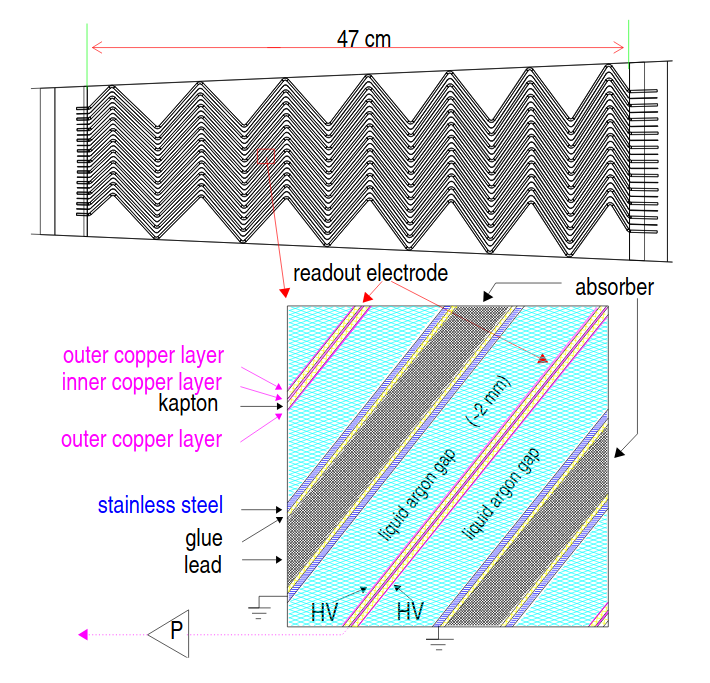
\includegraphics[width=0.6\textwidth]{Ch2/Img/ECal_accord.png}
    \caption{Accordion shape of the EM calorimeter.}
    \label{fig:chap2:ATLAS:Calo:ECal:Acc}
\end{figure}
\\
The ECal is further segmented in three longitudinal layers, to measure the longitudinal shower development. They are called respectively strip, middle, and back. It has different EM cells granularity $\Delta\eta\times\Delta\phi$ per layer. Cells of the middle layer (Lr2) in the barrel region have a size of 0.025$\times$0.025, while for the strip (Lr1) cells are 8 times finer in the $|\eta|$ direction providing a precise $\eta$ measurement of incident particles. The back layer (Lr3) cells has a twice coarser granularity in $\eta$ and the same $\phi$ segmentation as in Lr2. In front of the EM barrel calorimeter there is a Presampler (PS) LAr detector (Lr0), covering range $|\eta| < $ 1.8 and placed to start the shower before the calorimeter. PS has the finest granularity with a cell size of $\Delta\eta\times\Delta\phi =$  0.003$\times$0.1 used for $\pi\rightarrow\gamma\gamma$ background separation. The number of samplings  and the granularity in each of the samplings are summarized in Table \ref{tab:chap2:ATLAS:Calo:ECal:Gr}. \\
\begin{table}[htbp]
    \centering
    \begin{tabular}{lccccc}
    \hline
    Sampling & $|\eta| < $ 1.5 & 1.5 $ < |\eta| < $ 1.8 & 1.8 $ < |\eta| < $ 2.0 & 2.0 $ < |\eta| < $ 2.5 & 2.5 $ < |\eta| < $ 3.2 \\
    \hline
    \hline
        Presampling & 0.025$\times$0.1 & 0.025$\times$0.1  \\
        Strip & 0.025/8$\times$0.1 & 0.025/8$\times$0.1 & 0.025/6$\times$0.1 & 0.025/4$\times$0.1 & 0.1$\times$0.1 \\
        Middle & 0.025$\times$0.025 & 0.025$\times$0.025 & 0.025$\times$0.025 & 0.025$\times$0.025 & 0.1$\times$0.1 \\
        Back & 0.050$\times$0.025 & 0.05$\times$0.025 & 0.05$\times$0.025 & 0.05$\times$0.025 \\
        \hline
    \end{tabular}
    \caption{Granularity of the EM calorimeter ($\Delta\eta\times\Delta\phi$) \cite{LAr_TRD}.}
    \label{tab:chap2:ATLAS:Calo:ECal:Gr}
\end{table}
\\
The EM calorimeter energy resolution is given by:
\begin{equation}
    \sigma_E/E = \frac{10\%}{E} \oplus 0.7\%.
\end{equation}

\subsubsection{Hadronic calorimeter}
\label{chap2:ATLAS:Calo:HCAL}
 At high-energy colliders, quarks and gluons fragment into a shower of particles called jets. The Hadronic Calorimeter (HCal) completes the measurement of the jet energy initiated by the ECal \cite{Tile_TDR}. Hadronic showers are larger than electromagnetic ones, thus HCal needs to be large enough to contain the hadronic shower and reduce the punch-through hadrons penetrating to the muon system. The total thickness was chosen to be about 11 $X_0$ to obtain good performances on the resolution for high-energy jets. The hadronic calorimeter is divided into the Tile calorimeter and the LAr hadronic end-caps calorimeter. The barrel calorimeter is made of steel as absorbing material and scintillating plastic tiles as the active medium and covers the range $|\eta| < $ 1 with two extensions in the range 0.8 $ < |\eta| < $ 1.7. The end-caps cover the range 1.5 $ < |\eta| < $ 3.2, and they are composed of two wheels made of parallel copper plates with LAr as active material in between. For the determination of the missing energy, a good hermetic coverage is essential. Therefore, the ATLAS calorimeter is also equipped with a calorimeter covering the very forward region of 3.1 $ < |\eta| < $ 4.9, the LAr Forward Calorimeter (FCal). \\
 
\textbf{Tile} calorimeter provides signal by the tiles scintillation. Tiles are 3 mm thick and perpendicular to the beam pipe. It is consists of a barrel ($|\eta| < $ 1.0) and two extended barrels (0.8 $ < |\eta| < $ 1.7). The Tile calorimeter is segmented into three layers. The dimension of the cells corresponds to $\Delta\eta\times\Delta\phi=$ 0.1$\times$0.1 in the first two layers and $\Delta\eta\times\Delta\phi=$ 0.2$\times$0.1 in the last layer to contain the hadronic shower. A vertical gap of 68 cm wide between the barrel and extended barrel regions is used for the transition from the ID and the EM calorimeter. \\
 
 \textbf{LAr} cover end-cap and forward regions with 1.5 $ < |\eta| < $ 4.9. Each end-cap calorimeter (HEC) consists of two independent wheels of equal diameter with copper absorber plates. The end-cap calorimeter is divided into front, middle and back longitudinal layers. The FCal is placed at a distance of about 5 meters from the interaction point. It is a high-density detector facing a very high particle flux and consisting of three wheels on each side employing liquid argon as an active material. The innermost wheel is optimized for electromagnetic showers and employs copper as the absorber. While the other two wheels measure hadronic showers using tungsten as absorbing material. The granularity of the hadronic LAr calorimeter is $\Delta\eta\times\Delta\phi=$ 0.1$\times$0.1 for 1.5 $ < |\eta|< $ 2.5 and $\Delta\eta\times\Delta\phi=$ 0.2$\times$0.2 for 2.5 $ < |\eta| < $ 3.2 while the forward calorimeter has $\Delta\eta\times\Delta\phi=$ 0.2$\times$0.2.\\
 The HCal is designed to measure the energy with a resolution of \cite{Tile_Perf}:
 \begin{equation}
     \sigma_E/E = \frac{50\%}{E} \oplus 3\%.
 \end{equation}

\subsection{Muon Spectrometer}
\label{chap2:ATLAS:MS}
Muons are minimally ionizing particles due to their relatively high mass, therefore are not stopped by the calorimeter system. The Muon Spectrometer (MS) is the outermost part of the ATLAS detector dedicated to detect muons exiting the calorimeter and measure their momentum in the range of $|\eta| < $ 2.7 \cite{Muon_TDR}. A large superconducting air-cored toroid magnet is used to bend muons trajectories. Over the range of $|\eta| < $ 1.4, magnetic bending is provided by the large barrel toroid. For 1.6 $ < |\eta| < $ 2.7 region, muon tracks are bent by two smaller end-cap magnets inserted into both ends of the barrel toroid. Over 1.4 $ < |\eta| < $ 1.6, usually referred to as the transition region, magnetic deflection is provided by a combination of barrel and end-cap fields. Two different functions are accomplished by the MS: triggering and high-precision tracking. The tracking is performed by the Monitored Drift Tube (MDT) and by Cathode Strips Chamber (CSC) at large pseudo-rapidity. However, the trigger system covers the region up to $|\eta| < $ 2.4, and it is composed of Resistive Plate Chamber (RPC) in the barrel and Thin Gap Chamber (TGC) in the end-caps. The conceptual layout of the spectrometer is shown in Figures \ref{fig:chap2:ATLAS:MS}. \\
\begin{figure}[htbp]
    \centering
    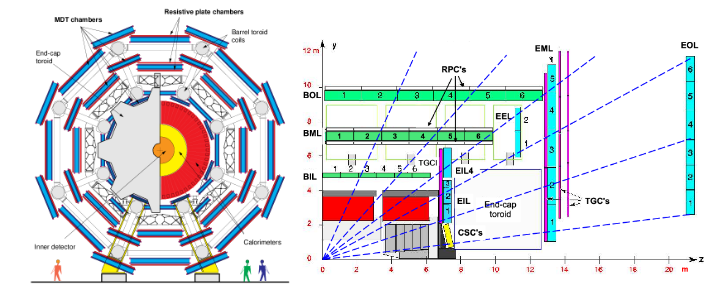
\includegraphics[width=0.75\textwidth]{Ch2/Img/Muon.png}
    \caption{Side view of one quadrant ($right$) and transverse view ($left$) of the muon spectrometer.}
    \label{fig:chap2:ATLAS:MS}
\end{figure}
\\
The MDTs are aluminium drift tubes with a diameter of 30 mm as Figure \ref{fig:chap2:ATLAS:MS:Tube} shows, operating with a gas mixture of 93\% of $Ar$ and 7\% of $CO_2$ at 3 bar pressure. Each chamber consists of two sections with three (inner station) or four (middle and outer station) layers of the drift tubes. Tungsten-rhenium wire of 50 $\mu$m collects the electrons resulting from ionization at a potential of 3 kV. The maximum drift time can reach about 700 ns. The MDTs are designed for precise tracking of muons and cover most of the MS pseudorapidity total coverage, with a single-hit resolution of about 35 $\mu$m per chamber. \\
\begin{figure}[htbp]
    \centering
    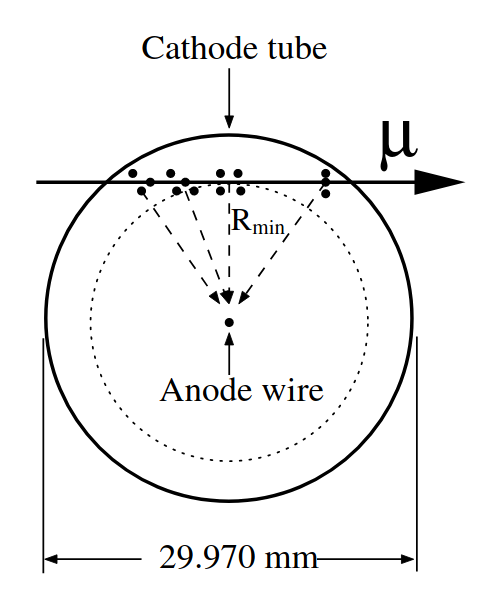
\includegraphics[width=0.35\textwidth]{Ch2/Img/Tube.png}
    \caption{Transverse cross-section of the MDT tube.}
    \label{fig:chap2:ATLAS:MS:Tube}
\end{figure}
CSCs are multi-wire proportional chambers filled with a mixture of 80\% of $Ar$ and 20\% of $CO_2$ with cathode planes segmented into strips in an orthogonal direction to the beam axis. The CSCs cover the range of 2.0 $ < |\eta| < $ 2.7 which is partially covered by the ID and has higher particle flux, because of their better time resolution and rate capability than MDTs. The CSC chambers have a slightly lower resolution than the MDTs, with 40 $\mu$m in the tracks bending plane, and 5 mm in the transverse plane. \\
For trigger purpose, the RPCs placed in the barrel, covering the range $|\eta| < $ 1.05,  are arranged into three concentric layers around the beam axis and placed before or after the MDT layers as Figure shows \ref{fig:chap2:ATLAS:MS}. The RPC unit is composed of a gap of 2 mm formed by two parallel electrodes. The gap is filled with a mixture gas of 94.7\% of $C_2H_2F_4$, 5\% of $Iso-C_2H_2F_4$ and 0.3\% of $SF_6$ $C_2H_2F_4$. The electric field between electrodes is about 4.9 kV/mm. The end-caps are equipped with the TGCs up to $|\eta| = $ 2.4. The TGCs are multi-wire proportional chambers filled with a mixture 55\% of $CO_2$ and 45\% of $n-C_5H_{12}$. The TGCs are arranged in seven layers on each side.\\
The overall momentum resolution $\frac{\sigma_{p_T}}{p_T}$ provided by the muon system is 4\% (1\%) at 5 GeV (1 TeV) \cite{ATLAS_Perf}.

\subsection{Trigger}
\label{chap2:ATLAS:Trigger}
The collision rate at the centre of ATLAS is 40 MHz due to the bunch crossing in every 25 ns provided by LHC. At such a rate, it is technically not possible to fully reconstruct, process and store all data recorded by the ATLAS detector. The ATLAS trigger system was designed to handle this problem. Its purpose  is to reduce the input of 40 MHz bunch crossing rate to an output rate of about 200 Hz to record them for offline analysis. This is done thanks to two separated trigger systems. The first level, so-called Level-1 (L1) \cite{Trigger_L1}, is a hardware-based trigger that uses reduced granularity signals from the calorimeter and the muon spectrometer to identify Regions-Of-Interest (ROI) with high-energy objects or high multiplicity at a latency of 2.5 $\mu$s. The L1 trigger system is responsible for reducing the rate to at least 75 kHz. Events passing the L1 trigger are then sent to the software-based High-Level Trigger (HLT) \cite{Trigger_HLT}. At the HLT, a fast analysis of the ROIs followed by an offline-like reconstruction of the events takes place with a processing time of around 0.2 s. The HLT creates an output with a frequency of around 1 kHz \cite{DQ}. For final states with large production rates, it can be necessary to keep only a fraction to match the offline storage budget.

\section{Upgrade plans towards Run-3 and the HL-LHC}
\label{chap2:Upgrad}
The long-term plan for the instantaneous luminosity delivered by the LHC foresees a step-wise increase due to continuous upgrades to the accelerator. To cope with the increased event rate and higher pile-up, the LHC experiments perform upgrades to various detector components, too. The main changes in the detector setup are performed during the long shutdown (LS) phases that are planned for 2019-20 (LS2 with the so-called Phase-1 upgrades) and 2025-27 (LS3 and Phase-2 upgrades). During LS2 and LS3, different detector and accelerator upgrades will be installed in ATLAS and LHC. After LS2, LHC could provide around 300 \ifb of data at the end of Run-3, and run with an increased centre-of-mass energy ($\sqrt{s} = $ 14 TeV). The Run-3 data taking was planned to start at the beginning of 2021, while given the coronavirus (Covid-19) epidemic the plan was delayed by 4 months (correspond to 4 months of quarantine).  A subsequent upgrade of the LHC (LS3), the so-called High-Luminosity (HL-LHC), would increase instantaneous luminosity and deliver around 3000 \ifb in 10 years.  An overview of the LHC operation plan is shown in Figure \ref{fig:chap2:Upgrad}. The mean pile-up is expected to be up to  $<\mu> = $ 200 during the HL-LHC operation. To cope with the more difficult conditions, the planned upgrades of ATLAS include replacement of the ID during the LS3 by the so-called ITk, a silicon detector made of pixels and strips. ITk will allow us to achieve at least similar tracking and vertex precision in the HL-LHC conditions. In addition to ITk, the planned upgrades also include a tracking system extension with the so-called High-Granularity Timing Detector (HGTD) \cite{HGTD}, based on low gain avalanche detector technology. HGTD will improve the identification of pile-up in the forward direction.  High-precision timing greatly improves the track-to-vertex association, leading to performance similar to that in the central region for the reconstruction of both jets and leptons, as well as for the tagging of heavy-flavour jets. These improvements in object reconstruction performance translate into important sensitivity gains and enhance the reach of the HL-LHC physics program, that double Higgs boson search would profit from it. The full ATLAS upgrade program can be found in the Ref. \cite{CERN-LHCC-2015-020, CERN-LHCC-2017-021, CERN-LHCC-2017-020, CERN-LHCC-2017-005, CERN-LHCC-2017-017, CERN-LHCC-2017-018, CERN-LHCC-2017-019}.

\begin{figure}[htbp]
    \centering
    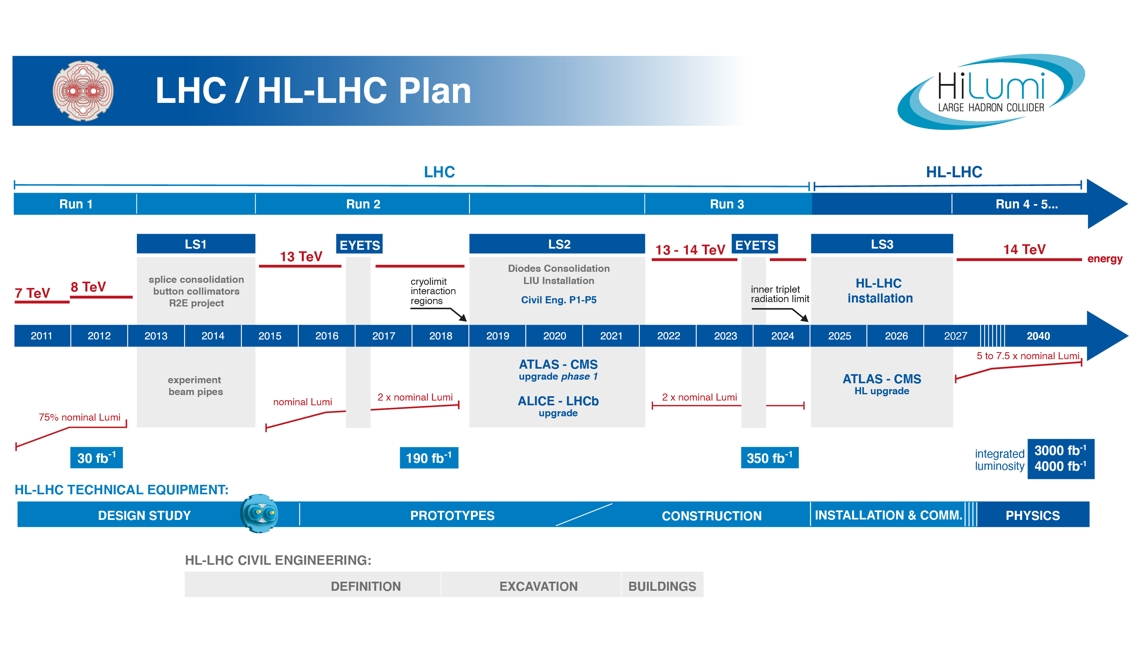
\includegraphics[width=0.75\textwidth]{Ch2/Img/HL-LHC-January-2021_small.jpg}
    \caption{Operation plan for the LHC scientific program.}
    \label{fig:chap2:Upgrad}
\end{figure}

\section{Physics objects reconstruction}
\label{chap2:Objects}
ATLAS provides energy deposits collected by sub-detectors. To interpret this raw output in terms of the event particles, an advanced particle reconstruction chains was developed. These are described in the following sections.

\subsection{Track and vertex reconstruction}
\label{chap2:Objects:Trk}
Tracks are reconstructed in the ID (Section \ref{chap2:ATLAS:ITk}) using a sequence of algorithms \cite{Track_Reco, New_Trk}. The inside-out algorithm starts from three points seeds in the SCT. A combinatorial Kalman filter (Iterative algorithm that provides the best estimate of the state based on the projection of earlier measurements and current measurement \cite{Kalman}) is used to build track candidates from the chosen seeds by incorporating additional space-points from the remaining layers of the PD and SCT which are compatible with the preliminary trajectory. Ambiguities in the track candidates are resolved, and tracks are extended into the TRT. The inside-out is the baseline algorithm designed for the efficient reconstruction of primary charged particles. In the second stage, a back-tracking algorithm is used in the track search starting from segments reconstructed in the TRT and extending them inwards by adding silicon hits. Back-tracking is designed to reconstruct secondary particles. \\
Finally, tracks with a TRT segment but no extension into the silicon detectors are referred to as TRT-standalone tracks. To minimize the rate of the fake track in a high pile-up environment, two-track quality requirements are defined. The robust requirement requests at least 9 hits in the silicon detectors and zero holes (non-existing but expected hit) in the PD. In contrast to the robust, the default requires at least 7 silicon hits and allow at most two-pixel holes.\\
The track reconstruction efficiency is defined as the fraction of primary particles with \pT $>$ 400 MeV and $|\eta|<$ 2.5 matched to a reconstructed track. Figure \ref{fig:chap2:Objects:Trk:Eff} shows the track reconstruction efficiency as a function of \pT and $\eta$.
\begin{figure}[htbp]
    \centering
    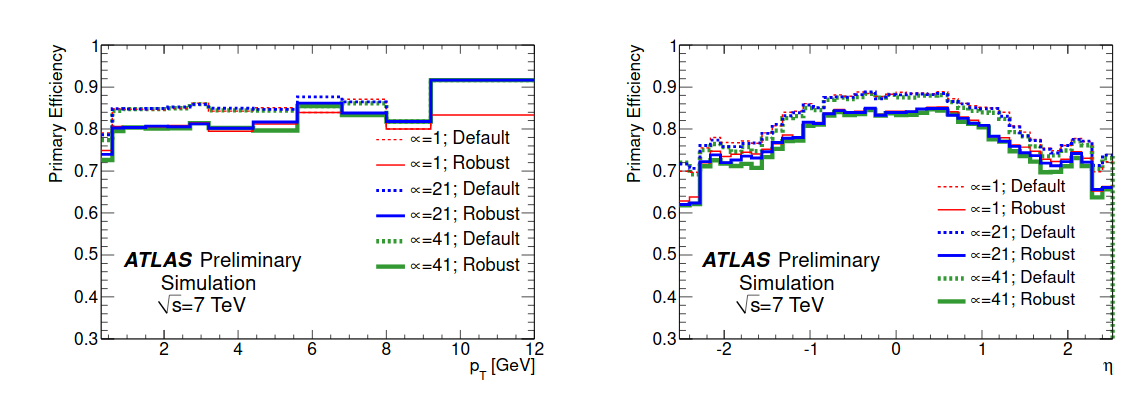
\includegraphics[width=0.9\textwidth]{Ch2/Img/Track_reco_eff.png}
    \caption{The primary track reconstruction efficiency in minimum bias simulated samples containing exactly one and on average 21 or 41 interactions. The distributions are shown for tracks passing the default(dashed) and robust (solid) requirements.}
    \label{fig:chap2:Objects:Trk:Eff}
\end{figure}
\\
Primary vertices are reconstructed using an iterative vertex finding algorithm \cite{Vrtx_Eff}. Vertex seeds are obtained from the z-position at the beam axis of the reconstructed tracks. An iterative $\chi^2$ fit constrained with the beam spot position is made using the seed and nearby tracks. Tracks are weighted depending on the $\chi^2$ to measure the compatibility with the fitted vertex \cite{chi2}. Tracks displaced by more than 7$\sigma$ from the vertex are used to seed a new vertex and the procedure is repeated until no additional vertex is found. During the reconstruction, vertices are required to contain at least two tracks. The efficiency to reconstruct a vertex from a minimum bias interaction is shown in Figure \ref{fig:chap2:Objects:Vtx:Eff}. Vertices are matched to interactions by calculating the sum of the weights of the tracks associated to the interaction vertex. 
\begin{figure}[htbp]
    \centering
    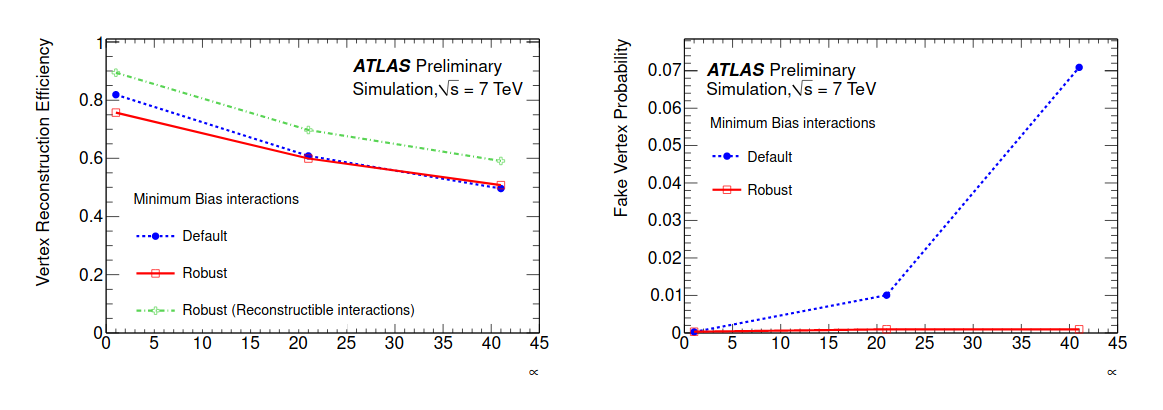
\includegraphics[width=0.9\textwidth]{Ch2/Img/Vtx_Reco_Eff.png}
    \caption{The vertex reconstruction efficiency ($left$) and fake probability ($right$) as a function of the average number of interactions.}
    \label{fig:chap2:Objects:Vtx:Eff}
\end{figure}

\subsection{Electron and photon reconstruction}
\label{chap2:Objects:Egamma}
Photons and Electrons are reconstructed similarly using the ECal (Section \ref{chap2:ATLAS:Calo:ECAL}). When these particles pass through the calorimeter dense medium, a showering process starts through cascading bremsstrahlung and electron pair production. The electrical signal induced by electrons from ionized active material (LAr) is proportional to the deposited energy in the active volume of the calorimeter and used to compute the cell energy. Note that, the cell energy is affected by fluctuations from both the electronic noise which is about 10 MeV per cell in the strip and 30 MeV in the middle and back layers and the pile-up noise. To reconstruct the EM clusters, the EM calorimeter is divided into a grid of $N_\eta\times N_\phi$ towers of the same granularity as the middle layer (0.025$\times$0.025). Inside each of these elements, the energy of all cells in all longitudinal layers is summed into tower energy. A window of fixed size 3$\times$5 is moved across each element of the tower. If the window transverse energy \eT (defined as the sum of the transverse energy of the towers contained in the window) is a local maximum and is above a threshold (2.5 GeV), a cluster seed is formed. Then, if the reconstructed cluster is associated with at least one reconstructed track, the candidate is classified as an electron. This reconstruction algorithm is called \textit{fixed-size} \cite{Fixed_size_cluster}. \\
A second reconstruction algorithm has been developed to benefit from dynamic, variable-size, clusters called \textit{super-clusters} \cite{Egamma_Perf_run2}. This allows the recovery of low-energy photons radiated due to bremsstrahlung interactions in the ID or electrons from photon conversions. In this scenario, the electron is defined as an object consisting of a supercluster and matched track. A converted photon is a cluster matched to a conversion vertex, and an unconverted photon is a cluster matched to neither an electron, track nor conversion vertex. In contrast to the sliding window (fixed-size), the super-cluster selects clusters based on topologically connected calorimeter cells \cite{Topo_cluster}. Figure \ref{fig:chap2:Objetcs:Egamma:SC} shows an illustration of super-clusters.  
\begin{figure}[htbp]
    \centering
    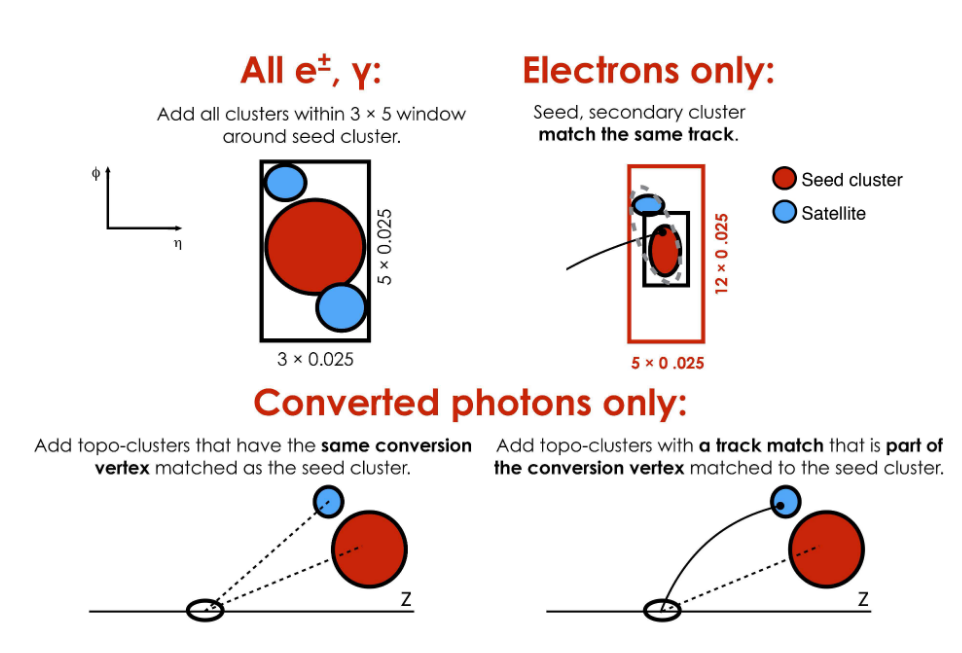
\includegraphics[width=0.7\textwidth]{Ch2/Img/Super_cluster.png}
    \caption{Diagram of the super clustering algorithm for electrons and photons. Seed clusters are shown in red, satellite clusters in blue.}
    \label{fig:chap2:Objetcs:Egamma:SC}
\end{figure}
The topological cluster reconstruction starts from a cell with $|E_{cell}|>$ 4$\sigma$, where $\sigma$ is the expected cell noise based on the known electronic noise and an estimation of the pile-up noise. Then successively, all neighbouring cells with $|E_{cell}|>$ 2$\sigma$ are added. The absolute cell energy is used to avoid biasing the cluster energy upwards due to negative energy induced by the calorimeter noise. The list of reconstructed topo-clusters is sorted according to descending total energy. The topo-clusters are tested one by one for use as a super-cluster. For an electron, the topo-cluster is required to have a minimum \eT of 1 GeV and matched to a track with at least four hits in the silicon detector \cite{GSF}, while for a photon the threshold is set to 1.5 GeV with no matched track or conversion vertex. For both cases, to recover radiative losses, satellite clusters around that reconstructed cluster are matched to the super-cluster. Tracks are matched to electron super clusters and conversion vertices to converted photon super clusters. The matching is performed in the same way as the matching to EM topo-clusters was performed, but using the super clusters instead. \\
The reconstruction efficiency using super clusters for an electron is shown in Figure \ref{fig:chap2:Objects:Egamma:El_Eff}.
\begin{figure}[htbp]
    \centering
    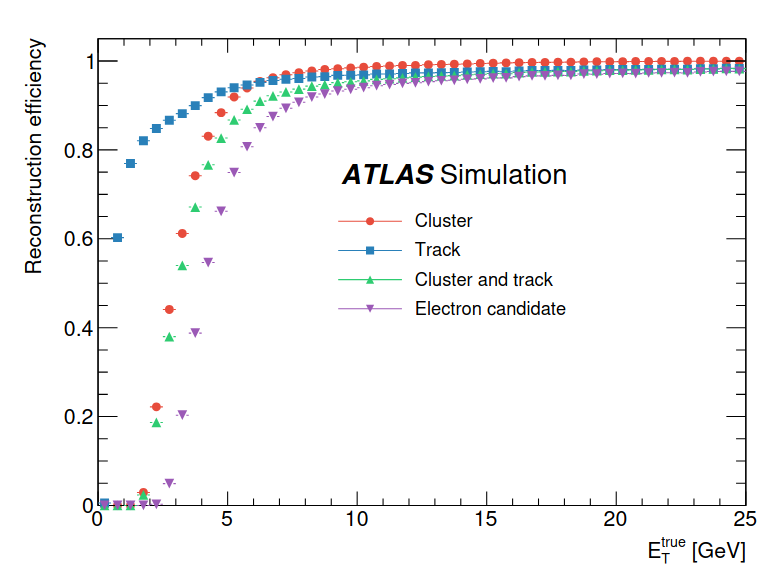
\includegraphics[width=0.5\textwidth]{Ch2/Img/Electron_Reco_Eff.png}
    \caption{The cluster, track, cluster and track, and electron reconstruction efficiencies as a function of the generated electron $E_T$.}
    \label{fig:chap2:Objects:Egamma:El_Eff}
\end{figure}
Figure \ref{fig:chap2:Objects:Egamma:Gamma:Conv:Reco:Eff} shows the reconstruction efficiency for converted photons as a function of the true \eT of the simulated photon for the previous version of the reconstruction software (fixed-size) and the current version (dynamic-size). An important reason for using super clusters is the improved energy resolution that super clusters provide by collecting more of the deposited energy.
\begin{figure}[htbp]
    \centering
    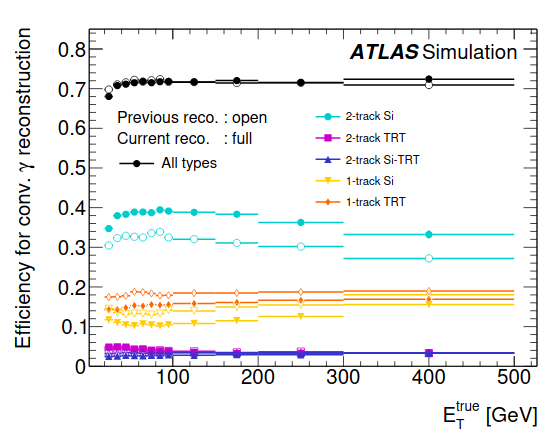
\includegraphics[width=0.5\textwidth]{Ch2/Img/Photon_conv_Reco_Eff.png}
    \caption{The converted photon reconstruction efficiency and contributions of the different conversion types as a function of $E^{true}_T$.}
    \label{fig:chap2:Objects:Egamma:Gamma:Conv:Reco:Eff}
\end{figure}
\\
Additionally, an ambiguity resolution is performed to remove a part of the overlap in case one object is reconstructed at the same time as electron and photon since electron and photon super clusters are built independently. However, in order to maintain a high reconstruction efficiency, a residual overlap is allowed to match physics analysis needs. Figure \ref{fig:chap2:Objects:Egamma:Ambg} shows the procedure used for ambiguity resolution. 
\begin{figure}[htbp]
    \centering
    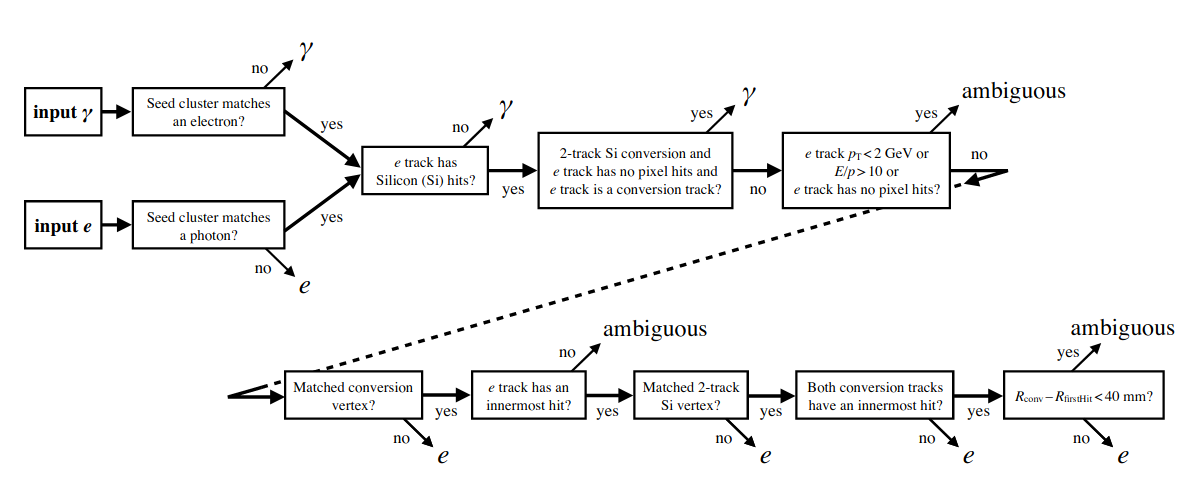
\includegraphics[width=0.8\textwidth]{Ch2/Img/Ambiguity.png}
    \caption{Flowchart showing the logic of the ambiguity resolution for particles initially reconstructed both as electrons and photons.}
    \label{fig:chap2:Objects:Egamma:Ambg}
\end{figure}
\\
Most LHC physics require the identification of prompt electrons and/or photons. Prompt particles are those not coming from a hadron or tau decay. Non-fake particles are those which type was properly reconstructed (i.e., a non-fake reconstructed electron is a true electron, not another misidentified particle). Their identification and separation are obtained with several selection criteria and algorithms. \\
The identification for the reconstructed electrons and photons is finally based on the reconstructed super-cluster objects. A set of discriminating variables are calculated for the identification using cells in the fixed-size window. A list is given in Table \ref{tab:chap2:Objects:Egamma:SS} long with an indication if they are used for electron or photon identification. The prompt and non-fake leptons/photons are usually isolated, without much activity around them. It is therefore important to define proper "isolation criteria" to reduce the contamination from non-prompt and fake objects. Electron isolation and identification are described in Sections \ref{chap2:Objects:Egamma:EIso} and \ref{chap2:Objects:Egamma:EID} respectively, while Chapter \ref{gamma} is dedicated to photon properties.
\begin{table}[htbp]
    \caption{Discriminating variables used for electron and photon
    identification. The usage column indicates if the variables are
    used for the identification of electrons, photons, or both. \cite{Egamma_Perf_run2}.}
   \def\arraystretch{1.3}
   \centering 
   \footnotesize
  \begin{tabular}{
  l
  >{\RaggedRight}p{0.55\textwidth}
  lc}
  \hline 
  \hline
  Category & Description & Name & Usage \\
  \hline 
  \hline
  Hadronic leakage
  & Ratio of $E_\mathrm{T}$ in the first layer of the hadronic calorimeter to $E_\mathrm{T}$ of the
    EM cluster (used over the ranges $|\eta|<0.8$ and $|\eta|>1.37$)  & $\Rhadone$ & $e/\gamma$  \\
  & Ratio of $E_\mathrm{T}$ in the hadronic calorimeter to $E_\mathrm{T}$ of the EM cluster
    (used over the range $0.8<|\eta|<1.37$)  & $\Rhad$  & $e/\gamma$ \\

  EM third layer
  & Ratio of the energy in the third layer to the total energy in the EM calorimeter & $\fIII$ & $e$ \\  

  EM second layer
  & Ratio of the sum of the energies of
  the cells contained in a $3\times7$ ($\eta\times\phi$)
  rectangle (measured in cell units)  to the sum of
  the cell energies in a $7\times7$ rectangle, both centred around the
  most energetic cell & $\Reta$ & $e/\gamma$ \\
  & Lateral shower width, $\sqrt{(\Sigma E_i \eta_i^2)/(\Sigma E_i)
    -((\Sigma E_i\eta_i)/(\Sigma E_i))^2}$, where $E_i$ is the energy
    and $\eta_i$ is the pseudorapidity of cell $i$ and the sum is calculated within a window of $3\times5$ cells
     & $\wetatwo$ & $e/\gamma$ \\
  & Ratio of the sum of the energies of
  the cells contained in a $3\times3$ ($\eta\times\phi$)
  rectangle (measured in cell units) to the sum of
  the cell energies in a $3\times7$ rectangle, both centred around the
  most energetic cell  & $\Rphi$ & $e/\gamma$ \\

  EM first layer
  & Total lateral shower width, $\sqrt{(\Sigma E_i
    (i-i_\mathrm{max})^2)/(\Sigma E_i)}$, where $i$ runs over all
    cells in a window of $\Delta\eta \approx 0.0625$ and
    $i_{\textrm{max}}$ is the index of the highest-energy cell
     & $\wtot$ & $e/\gamma$ \\
  & Lateral shower width,
    $\sqrt{(\Sigma E_i (i - i_{\textrm{max}})^2)/(\Sigma E_i)}$,
    where $i$ runs over all cells in a window of 3 cells around the
    highest-energy cell & $\wthree$ & $\gamma$ \\
  & Energy fraction outside core of three central cells, within seven cells   & $\Fside$ & $\gamma$ \\
  & Difference between the energy of the cell associated with the
    second maximum, and the energy reconstructed
    in the cell with the smallest value found between the first and
    second maxima  & $\DeltaE$ & $\gamma$ \\
  & Ratio of the energy difference between the maximum energy deposit and the energy deposit in a secondary maximum in the cluster to the sum of these energies   & $\Eratio$ & $e/\gamma$ \\
  & Ratio of the energy measured in the first layer of the electromagnetic calorimeter to the total energy of the
    EM cluster & $\fI$ & $e/\gamma$ \\

    Track conditions
           & Number of hits in the innermost pixel layer &   $n_\mathrm{innermost}$ & $e$ \\
           & Number of hits in the pixel detector        &    $n_\mathrm{Pixel}$ & $e$ \\
           & Total number of hits in the pixel and SCT detectors  &   $n_{\mathrm{Si}}$  & $e$ \\
           & Transverse impact parameter relative to the beam-line &  \trackdO  & $e$ \\
           & Significance of transverse impact parameter defined as
              the ratio of \trackdO to its uncertainty &  $|\dOSignificance|$  & $e$  \\
           &  Momentum lost by the track between the perigee and the last measurement point divided by
             the momentum at perigee& \deltapoverp & $e$ \\
           & Likelihood probability based on transition radiation in the TRT &   \TRTPID & $e$  \\
    Track--cluster matching
           & $\Delta\eta$ between the cluster position in the first layer 
             of the EM calorimeter and the extrapolated track &   \deltaeta & $e$  \\
           & $\Delta\phi$ between the cluster position in the second layer
             of the EM calorimeter and the momentum-rescaled track,
             extrapolated from the perigee, times the charge $q$ & \deltaphires & $e$  \\
            &  Ratio of the cluster energy to the measured track momentum  &       $E/p$   &  $e$ \\
  \hline 
  \hline
  \end{tabular}
  \label{tab:chap2:Objects:Egamma:SS}
\end{table}

\subsubsection{Electron and Photon calibration}
\label{chap2:Objects:Egamma:Cal}
After the electron and photon super clusters are built, initial energy calibration and position correction are applied to them \cite{Egamma_Calibration}. A complex chain with several successive calibration steps is used to calibrate the electron and photon energies based on simulation and well-known reference processes. A schematic overview of the whole calibration chain is shown in Figure \ref{fig:chap2:Objects:Egamma:Cal}.
\begin{figure}[htbp]
    \centering
    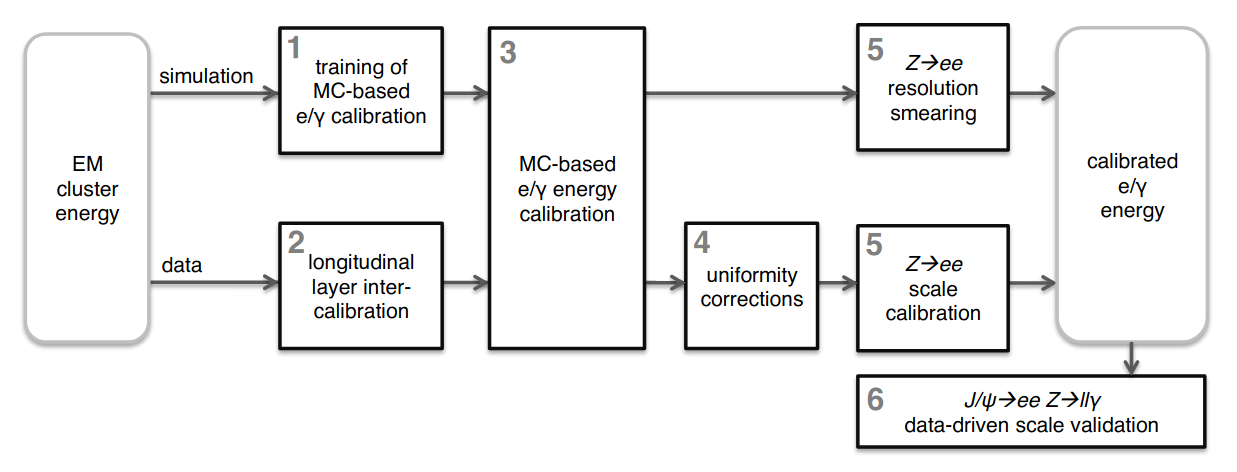
\includegraphics[width=0.6\textwidth]{Ch2/Img/Calibration_Chain.png}
    \caption{Schematic overview of the calibration chain for the electron and photon energies \cite{Egamma_Calib_run1}.}
    \label{fig:chap2:Objects:Egamma:Cal}
\end{figure}
\\
The calibration steps are:
\begin{enumerate}
    \item A multivariate regression algorithm is trained on the properties of the shower development in the EM calorimeter to optimize the energy resolution and to minimize the impact of material in front of the calorimeter. The algorithm used in this step is the Boosted Decision Tree (BDT) tuned in intervals of $|\eta|$ and $E_T$ on samples of simulated single particles without pile-up, separately for electrons, converted and unconverted photons. 
    \item An inter-layer correction is applied to the relative energy response in data to match the relative response in simulation in different calorimeter layers. The inter-layer calibration is independent of the material upstream of the calorimeter.
    \item The BDT correction is applied to both data and simulation. This step performs the main correction of the absolute energy scale and improves significantly the energy resolution.
    \item The non-simulated detector non-uniformities are therefore corrected in data. Correcting the effects of energy loss between the barrel calorimeter modules and the high-voltage inhomogeneities.
    \item Scale factors are applied to the energy in data to correct for the residual miscalibration between data and simulation using $Z\rightarrow e^+e^-$ events.
    \item The validity of the calibration is cross-checked from data using different processes. For the low-energy range, $J/\Psi\rightarrow e^+e^-$ events are used. The calibration for photons is cross-checked using radiative $Z\rightarrow l^+l^-\gamma$ ($l=e,\mu$) decays.
\end{enumerate}

\subsubsection{Electron Isolation}
\label{chap2:Objects:Egamma:EIso}
The activity near leptons and photons is quantified from the tracks of nearby charged particles or energy deposits in the calorimeters, leading to two classes of isolation variables, calorimeter-based isolation $E^{coneXX}_{T}$ and track-based $p_T^{coneXX}$ \cite{Electron_Reco_Id_Run1}. The corrected $E^{coneXX}_{T}$ is computed as the sum of the transverse energies of topo-clusters inside a cone of $\Delta R = \frac{XX}{100}$ around the reconstructed electrons. This is illustrated in Figure \ref{fig:chap2:Objects:Egamma:EIso:Schema}, after subtraction of the energy deposited by the electrons, pile-up and underlying event \cite{pile-up_IsoExtract}. $p_T^{coneXX}$ is the sum of the transverse momentum of selected tracks of \pT $>$ 1 GeV and $|\eta|<$ 2.5, within a cone centred around the electron track. Tracks matched to the electron are excluded. In a high-momentum heavy particles decay, the electron is produced very close to other decay products for this reason, an isolation $p_T^{varconeXX}$ with a variable cone size $\Delta R^{XX}$ is defined as:
\begin{equation}
    \Delta R^{XX} = min(\frac{10}{p_T[GeV]}, \frac{XX}{100}).
\end{equation}
\begin{figure}[htbp]
    \centering
    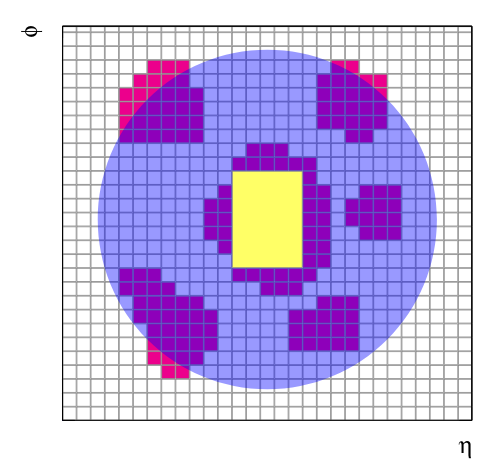
\includegraphics[width=0.5\textwidth]{Ch2/Img/Iso_Schema.png}
    \caption{Schema of the calorimeter isolation method: the grid represents the second-layer calorimeter cells in the $\eta$ and $\phi$ directions. The candidate electron is located in the centre of the purple circle representing the isolation cone. All topological clusters, represented in red, for which the barycentres fall within the isolation cone are included in the computation of the isolation variable. The 5$\times$7 cells represented by the yellow rectangle correspond to the subtracted cells in the core subtraction method.}
    \label{fig:chap2:Objects:Egamma:EIso:Schema}
\end{figure}
\\
Based on these variables, three different selection criteria, called working point (WP), are implemented. The WPs were defined in two different ways, either targeting a fixed value of efficiency or with fixed cuts on the isolation variables. Table \ref{tab:chap2:Objects:Egamma:EIso:WPs} lists the different electron-isolation WPs used in ATLAS.
\begin{table}[htbp]
    \centering
    \begin{tabular}{lcc}
    \hline \hline
        WP & Calorimeter-based isolation & Track-based isolation \\ \hline 
        \texttt{HighPtCaloOnly} & $E^{cone20}_T < max(0.015\times p_T, 3.5 GeV)$ & - \\
        \texttt{Loose} & $E^{cone20}_T/p_T < 0.2$ & $p^{varcone20}_T/p_T < 0.15$ \\
        \texttt{Tight} & $E^{cone20}_T/p_T < 0.06$ & $p^{varcone20}_T/p_T < 0.06$ \\ \hline \hline
    \end{tabular}
    \caption{Definition of the electron isolation WPs.}
    \label{tab:chap2:Objects:Egamma:EIso:WPs}
\end{table}
An additional WP named \texttt{Gradient} is designed to give an efficiency of 90\% at \pT = 25 GeV and 99\% at 60 GeV, uniform in $\eta$.\\
Figure \ref{fig:chap2:Objects:Egamma:EIso:Eff} shows the electron isolation efficiency in data recorded in 2017 as a function of electron \eT \cite{Egamma_Perf_2017}. The method used to compute the electron isolation efficiency and the associated uncertainties are described in Ref. \cite{Electron_Reco_Id_Run1}. The jump observed in Gradient efficiency at 15 GeV is due to the isolation efficiency which is process dependent: the Gradient cut maps is optimized with $J/\Psi\rightarrow e^+e^-$ events below 15 GeV, while the efficiency measurement is performed with $Z\rightarrow e^+e^-$.
\begin{figure}[htbp]
    \centering
    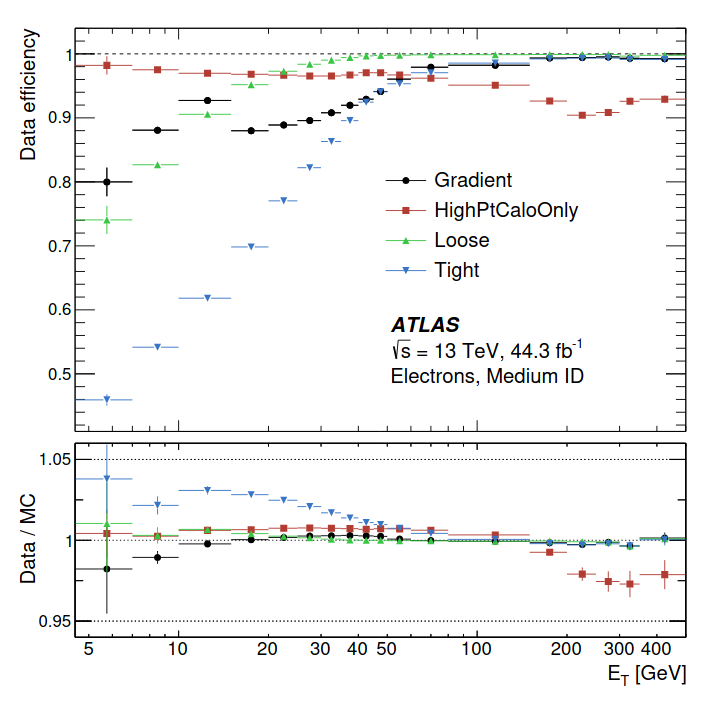
\includegraphics[width=0.5\textwidth]{Ch2/Img/Electron_Iso_Eff.png}
    \caption{Efficiency of the different isolation WPs for electrons from inclusive $Z\rightarrow e^+e^-$ events as a function of the electron \eT. The lower panel shows the ratio of the efficiencies measured in data and in simulations \cite{Egamma_Perf_2017}.}
    \label{fig:chap2:Objects:Egamma:EIso:Eff}
\end{figure}

\subsubsection{Electron Identification}
\label{chap2:Objects:Egamma:EID}
The identification of prompt electrons relies on a likelihood (LH) discriminant constructed from quantities measured in the different sub-detectors and listed in Table \ref{tab:chap2:Objects:Egamma:SS}. The electron LH is based on the products of the probability density functions (pdf) for signal $L_S$, and for background $L_B$. The PDFs are created by smoothing histograms of the n discriminating variables with an adaptive kernel density estimator (KDE) \cite{KDE} as implemented in the TMVA framework \cite{TMVA} in 9 bins of $|\eta|$ and 7 bins of \eT:
\begin{equation}
    L_{S(B)}(\textbf{x}) = \displaystyle\prod_{i=1}^{n} P_{S(B),i}(x_i),
\end{equation}
where \textbf{x} is the vector of the various variables. For each electron candidate, a discriminant $d_L$ is formed using an inverse sigmoid function transformation:
\begin{equation}
    d_L = -\frac{1}{\tau}ln(\frac{L_S+L_B}{L_S} - 1),
\end{equation}
where $\tau$ is fixed to 15 \cite{TMVA}. Figure \ref{fig:chap2:Objects:Egamma:EID:LH} shows an example of the distribution of the transformed discriminant for prompt electrons and non-prompt ones. This distribution illustrates the effective separation between signal and background encapsulated in this single quantity.
\begin{figure}[htbp]
    \centering
    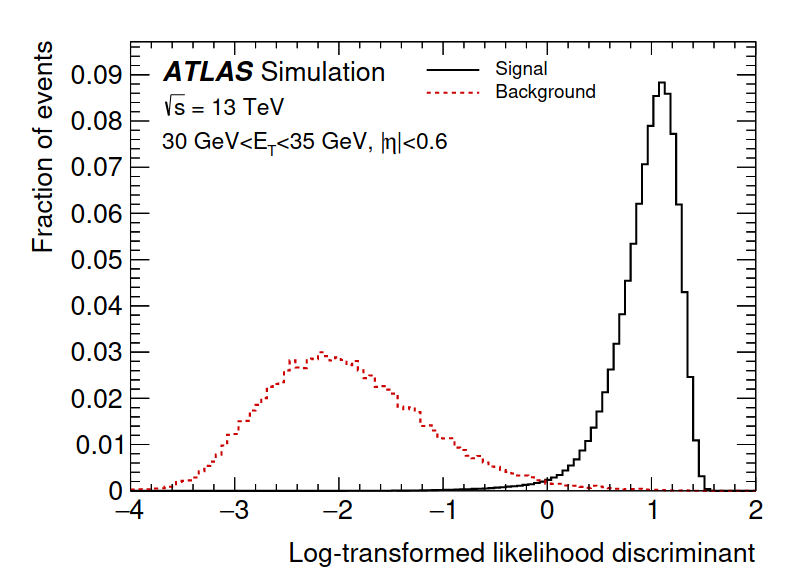
\includegraphics[width=0.5\textwidth]{Ch2/Img/Electron_LH.png}
    \caption{The transformed LH-based identification discriminant $d_L$ for reconstructed electron candidates with good quality tracks with 30 $ < E_T < $ 35 GeV and $|\eta|<$ 0.6 \cite{Electron_ID_2016}.}
    \label{fig:chap2:Objects:Egamma:EID:LH}
\end{figure}
\\
For physics purposes, three WPs are defined, and are referred to as \texttt{Loose}, \texttt{Medium}, and \texttt{Tight}. Their efficiency for identifying a prompt election with \eT = 40 GeV are 93\%, 88\% and 80\% respectively. Figure \ref{fig:chap2:Objects:Egamma:EID:Eff} shows the resulting efficiencies in data \cite{Egamma_Perf_run2}.
\begin{figure}[htbp]
    \centering
    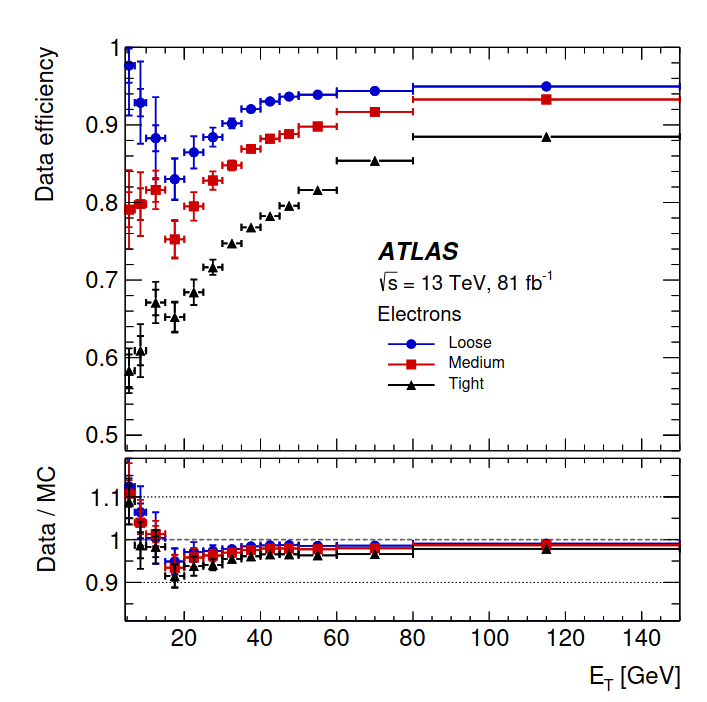
\includegraphics[width=0.5\textwidth]{Ch2/Img/Electron_ID_Eff.png}
    \caption{The electron identification efficiency in $Z\rightarrow e^+e^-$ events in data as a function of \eT for the \texttt{Loose}, \texttt{Medium}, and \texttt{Tight} WPs.}
    \label{fig:chap2:Objects:Egamma:EID:Eff}
\end{figure}

\subsection{Muon reconstruction and identification}
\label{chap2:Objects:Muon}
\subsubsection{Muon reconstruction}
\label{chap2:Objects:Muon:Reco}
Muon reconstruction is performed in two sub-detectors independently. Firstly, the muon tracks are reconstructed in the ID like any track as described in Section \ref{chap2:Objects:Trk}. Then, the ID reconstruction is combined with the muon reconstruction in MS sub-detector to perform the muon object used in physics analysis. In the MS, the muons are triggered in RPC/TGC if at least one hit exists, defining the region of activity (ROA). All the muon chambers intersecting with the ROA are then selected as muon track candidates. The MDT segments are reconstructed by performing a straight-line fit (the bending of muons larger than few GeV is sufficiently small) to the hits found in each layer \cite{hough}. The fitted segments are required to point loosely towards the IP, to reject background events and random hit combinations. Muon track candidates are then built by extrapolating each of these segments to the other. At least two matching segments using their relative positions and angles are required to build a track, except in the barrel–endcap transition region where a single high-quality segment can be used. \\
The combined reconstruction is performed according to various algorithms based on the provided information by sub-detectors \cite{Muon_Reco_2014_algo,Muon_Reco_2016_algo}: 
\begin{itemize}
    \item Combined (CB) muon: the combined muon is formed with a global refit that used the hits from both the ID and MS sub-detectors. The reconstruction is done following two complementary approaches, the outside-in in which the reconstructed track in the MS are extrapolated inward and match to an ID track, and the inside-out reconstruction, in which ID tracks are extrapolated outward and matched to MS tracks.
    \item Segment-tagged (ST) muon: used when muons cross only one layer of MS chamber, either because of their low \pT or because of MS acceptance. 
    \item Calorimeter-tagged (CT) muon: reconstructed track with an energy deposit in the calorimeter compatible with a minimum-ionizing particle is identified as CT muon. 
    \item Extrapolated (ME) muon: reconstructed based only on the MS track and a loose requirement on compatibility with originating from the IP. 
\end{itemize}
Overlaps between different muon types are resolved with preferences to CB, ST and CT muons respectively before producing the collection of muons used in physics analyses.

\subsubsection{Muon identification}
\label{chap2:Objects:Muon:ID}
In order to suppress non-prompt muons, mainly coming from pion and kaon decay, a muon identification is performed. Muon identification uses several variables, for CB tracks:
\begin{itemize}
    \item $q/p \ significance$ defined as: 
    \begin{equation}
        q / p \ significance=\frac{\left|q / p_{\mathrm{ID}}-q / p_{\mathrm{MS}}\right|}{\sqrt{\sigma^{2}\left(q / p_{\mathrm{ID}}\right)+\sigma^{2}\left(q / p_{\mathrm{MS}}\right)}},
    \end{equation}
    where $q/p_{ID}$ and $q/p_{MS}$ are the measurements in the ID and MS of the ratio of the charge $q$ to the momentum $p$ of the muon, expressed at the IP and $\sigma$ is the corresponding uncertainties. 
    \item $\rho'$ defined as the absolute value of the difference between the transverse momentum measurements in the ID and MS divided by the \pT of the combined track.
    \item Normalized $\chi^2$ of the combined track fit. 
\end{itemize}

Four muon identification WPs are provided to address specific needs of different physics analysis:
\begin{itemize}
    \item \texttt{Loose}: designed to maximize the reconstruction efficiency while providing good-quality muon tracks. They are specifically optimized for reconstructing Higgs boson candidates in the four-lepton final state \cite{Higgs_4leptons}.
    \item \texttt{Medium}: provides the default selection for muons in ATLAS. This selection minimizes the systematic uncertainties associated with muon reconstruction and calibration. Only CB and ME tracks are used. About 0.5\% of Medium muon originates from the inside-out reconstruction strategy, in the central region. 
    \item \texttt{Tight}: maximizes the purity of muons at the cost of efficiency. Only CB muons with hits in at least two stations of the MS and satisfying the \texttt{Medium} selection criteria are considered.
    \item \texttt{High-$p_T$}: aims to maximize the momentum resolution for tracks with transverse momentum above 100 GeV. The selection is optimized for searches for high-mass Z' and W' resonances \cite{W,dilepton}. CB muons passing the \texttt{Medium} selection and having at least three hits in three MS stations are selected.
\end{itemize}
Figure \ref{fig:chap2:Objects:Muon:ID:Eff} shows the muon identification efficiency for \texttt{Loose}, \texttt{Medium} and \texttt{Tight} muons as measured in $J/\Psi\rightarrow\mu\mu$. 
\begin{figure}[htbp]
    \centering
    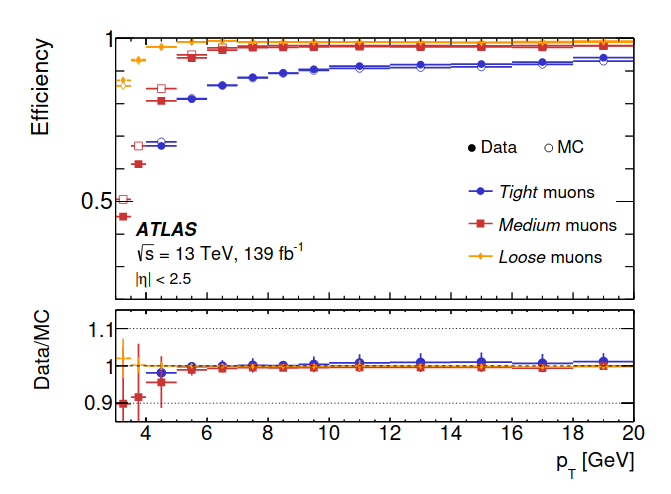
\includegraphics[width=0.5\textwidth]{Ch2/Img/Muon_ID_Eff.png}
    \caption{Muon identification efficiency for the \texttt{Loose}, \texttt{Medium} and \texttt{Tight} WPs as function of \pT. The panel at the bottom shows the ratio of the measured to predicted efficiencies, with statistical and systematic uncertainties.}
    \label{fig:chap2:Objects:Muon:ID:Eff}
\end{figure}

\subsection{Jet reconstruction}
\label{chap2:Objects:Jet}
Jets are made of many partons coming from the initial quark or gluon hadronization, appearing in the detector as a collimated shower. Many jets reconstruction algorithms exist in ATLAS, but only two approaches are of interest for the work presented in this thesis. The first approach is based exclusively on electromagnetic and hadronic topological clusters, so-called EMTopo jets. The second approach uses both tracking and calorimetric information through a Particle Flow algorithm to build PFlow jets \cite{Jet_Perf_Run2}. Jets are reconstructed using the anti-$k_t$ algorithm \cite{Anti-Kt}, with a distance parameter of R = 0.4. Jets reconstruction, calibration and identification of $b$-jets will be discussed in more details in Chapter \ref{Jet}. 

\subsection{Missing transverse energy}
\label{chap2:Objects:MET}
Neutrinos and other BSM particles interact extremely weakly with matter, making them hard to detect, and they cannot be observed directly as hadrons, electrons or muons discussed before. Their energy is reconstructed as missing transverse energy (MET). Thanks to momentum conservation, the transverse momentum of all particles generated in a collision should sum up to zero, since the original transverse momentum of the partons is negligible. MET is defined as the sum of the transverse energy momenta of all reconstructed objects $i$: 
\begin{equation}
    \vec{E}_{T}^{m i s s}=-\sum_{i} \vec{p}_{T}^{i}
\end{equation}
The MET resolution is typically 10-20 GeV \cite{MET_reso}.